\documentclass{article}
%\documentclass{ctexart}
\usepackage{multicol}
\usepackage{wrapfig}
\usepackage{lipsum}
%\documentclass{ctexart}
\usepackage{ctex}%中文
\usepackage{graphicx}
\usepackage{zhlipsum}
\usepackage{multirow}
\usepackage{cuted}
\graphicspath{{picture/}}
\usepackage[left=2.5cm,right=1.97cm,top=2.5cm,bottom=2.5cm]{geometry}%设置页边距
\renewcommand{\baselinestretch}{1.25}%行间距
\usepackage[hidelinks,urlcolor=black,linkcolor=black]{hyperref}%引入超链接包,否则会出现Undefined sequence
%[colorlinks,urlcolor=black,linkcolor=black]去除超链接中的颜色框
\usepackage{amssymb}%数学符号
\usepackage{amsmath}%数学公式
\usepackage{booktabs}%设置三线表的线粗细
\usepackage{array}%table
\newcommand{\tabincell}[2]{\begin{tabular}{@{}#1@{}}#2\end{tabular}}
\usepackage{cite}
% \ctexset{section={format={\zihao{3} \heiti \bfseries}},
% bibname={\zihao{-4} \heiti \bfseries 参考文献}}

\newcommand{\upcite}[1]{\textsuperscript{\textsuperscript{\cite{#1}}}}


\title{\heiti \zihao{2} 基于深度学习的机器阅读理解技术研究综述}%黑体2号 在标题那页插入脚注



\author{\kaishu \zihao{-4} 孙相会\\
\songti \zihao{-5} 学号:1971654}%-4就是小四号
\date{}
%%%%%%%%%%%%%%%%%%%%%%%%%%%%%%%%%%%%%%%
\begin{document}
    \maketitle %生成title,author,date

        \noindent \textbf{摘\quad 要}: 机器阅读理解
的目的是使得机器能够理解自然语言文本,
它是自然语言处理领域
十分重要的研究方向。
随着深度学习技术的进步以及大规模数据集的发布,在机器阅读理解方向
上的研究已经取得了很大的突破。近年来随着自然语言处理领域预训练模型的出现,再一次推动了机器阅读理解领域的发展。
本文主要从四个方面对自2015年以来机器阅读理解领域的发展做综述:介绍机器阅读理解的任务定义以及相关数据集;
分析机器阅读理解领域经典的基于注意力机制或推理结构的模型以及目前流行的预训练模型;
探讨更加复杂的机器阅读理解任务;
总结机器阅读理解领域目前存在的问题并且对未来的研究趋势做展望。\\
\heiti 关键词: \songti 机器阅读理解;自然语言处理;预训练模型;注意力机制;推理结构 \\
%\heiti 中图分类号: \songti ? \hspace{1cm} \heiti 文献表示码: \songti A \\
\textbf{文献标识码:} A  \qquad \textbf{中图分类号:} TP391
\begin{center}
    \textbf{\zihao{4} Overview of Studies on Neural Machine Reading Comprehension \\}

%     \zihao{5} Xianghui Sun \\
% \zihao{-5} id: 1971654 (NEU) 
%\zihao{-4} SUN Xianghui \\
%College of Computer Science and Engineering,Northeasten University,Shengyang 110169,China

\end{center}
\textbf{Abstract:} Machine Reading Comprehension aims to make machines comprehend the natural language documents, which 
is an important research direction
 in the field of natural language processing. With the development of deep learning technology and release of large scale datasets, the research on the field of machine reading comprehension has made great breakthroughs. 
 With the emergence of pre-trained model in natural language processing in recently years, it promotes the development of machine reading comprehension once again. This paper mainly make a survey from four aspects over the development of machine reading comprehension in recently years: to introduce the definition of 
  machine reading comprehension tasks and its corresponding datasets; to analyze classical model in the field of machine reading comprehension  
  which based on attention mechanism or reasoning structure as well as the currently 
  popular pre-trained model; to discuss more complicated machine reading comprehension tasks;
   to summarize the existing problem and look into the future research trend about machine reading comprehension. \\
\textbf{Key words:} machine reading comprehension; natural language processing; pre-trained model; attention mechanism; reasoning structure












    what
    \url{https://blog.csdn.net/
    }
%----------------------正文-----------------------
\begin{multicols}{2}
    \section{引言}

%\vspace{10cm}在垂直方向上,两行之间的距离
机器阅读理解(MRC)是自然语言处理领域十分重要也是具有挑战性的研究方向,这项任务的目的是衡量计算机理解自然语言文本的能力。具体的就是
给定一篇文章和相关的问题,要求计算机通过阅读理解这篇文章后能够正确的回答这些问题。早期的MRC系统主要是基于规则和模式匹配的方法,
而且数据集规模比较小,系统难以获得期望的性能也不能实际的应用。随着深度学习的兴起,词嵌入技术的发展,注意力机制应用在NLP领域\cite{neural machine translation by jointly learning to align and translate}以及
大规模阅读理解数据集如(CNN/Daily Mail\cite{Teaching Machines to Read and Comprehend},SQuAD\cite{SQuAD1},
RACE\cite{RACE},MS MARCO\cite{MS marco},CoQA\cite{CoQA}等)的发布,
这些推动了MRC领域的发展,越来越多的学者采用神经网络构建MRC模型,也叫神经机器阅读理解,效果上显著的优于传统的机器学习方法并且在
SQuAD\cite{SQuAD1}数据集上逐渐的接近人类的阅读理解水平。

自2018年,随着ELMo\cite{ELMo}、GPT\cite{GPT}、BERT\cite{BERT}等预训练语言模型的出现,再一次提升了机器阅读理解的水平,
特别是BERT\cite{BERT}在SQuAD数据集上首次超过了人类的表现。

本篇论文主要从具体任务,数据集,经典的神经机器阅读理解模型,目前流行的基于预训练的模型,对于不同任务的不同的评估指标以及MRC领域
目前新的趋势几方面对机器阅读理解领域做阐述。

\end{multicols}
%在你想要分栏的段落上下加上begin end columns{2}
%\section{机器阅读理解任务概述}

%\footnotetext[1]{\url{www.cnn.com}}\label{1}\vspace{-10pt}
机器阅读理解(MRC)任务是为了使得计算机具有对自然语言文本理解的能力,像人类一样阅读并且理解一篇文章。
MRC可以用一个三元组$<D,Q,A>$来描述,其中$D$代表文章(Document)\footnote{本文中文章(Document)和段落(Passage)是同样的概念},$Q$表示问题(Question),$A$表示答案(Answer),即
给定一篇文章$D$和一些与文章$D$相关的问题$Q$,
要求模型通过阅读$D$之后给出$Q$的正确答案$A$,建模给定$D$和$Q$的条件下预测$A$的概率:$P(A|D,Q)$
。

MRC任务已经从早期的需要阅读一篇文章,答案是单个单词的阅读理解任务,发展到需要阅读多篇文章,并且答案需要从多篇文章中推理出来的阅读理解任务,使得阅读理解任务更加的贴近真实场景。
%甚至只需某个相关的上下文句子即可正确的填写出问题中的单词。经过近几年的MRC领域的快速发展,目前已经有很多数据集既需要模型从多篇文章中多步推理又要同时给出不限于文章中单词的答案,任务的难度显著上升。
本文按照Chen\upcite{base}
提出的分类方式,根据答案形式的不同将阅读理解任务概括为4类任务:填空式、多项选择式、抽取式和自由答案式。
%随着近年来MRC领域的发展出现了一些新兴的阅读理解任务如带有无答案问题的任务,对话形式的任务等,本文将机器阅读理解任务划分为yixia
下面对这四种类型任务分别进行叙述并介绍相关的数据集。



\subsection{填空式}
填空式阅读理解是指给定一篇文章$D$和一个与文章相关的问题$Q$,$Q$是通过删除
掉句子中某一个单词构成,要求模型根据$D$能够
正确的填写出$Q$缺失的单词$a$,且$a\in D$。填空型数据集的一个样例见表1。

典型的填空式数据集是由Google DeepMind和牛津大学发布于2015年的CNN\&Daily Mail\upcite{CNNDailyMail}数据集,
这是第一个较大规模的完形填空型阅读理解型数据集。从CNN\footnote{www.cnn.com\label{cnn}}中收集93k篇文章,从
Daily Mail\footnote{www.dailymail.co.uk\label{daily mail}}上收集220k篇文章。删去句子中的一个命名实体单词,
以此作为问题,构建了(文章-问题-答案)的三元组形式的语料库作为填空式的阅读理解任务。

相关的数据集还有
Hill等人\upcite{CBT}发布了(Children's Book Test,CBT)数据集,语料库来源于儿童读物(Gutenberg\footnote{https://www.gutenberg.org/\label{cbt}}工程)。与CNN\&Daily Mail的不同之处是删除的单词不局限于命名实体,还可能删除句子中的名词、动词和介词。
%每一篇文章是由20个连续的句子构成,删除第21个句子中的某个单词作为问题。
CLOTH\upcite{CLOTH}数据集是收集自中国中学生的英语考试试题中的完型填空题型。
%与之前的填空型数据集最大的不同是问题中删除的单词不像之前数据集的构建方式那样是由系统根据规则自动构建的,这样生成的问题往往没有目的性并且答案可能会出现歧义。
每一个问题是由专家为了测验学生英语水平而精心设计的,空白处位置的单词通常会考察学生的词汇、语法以及推理能力,因此CLOTH数据集相比于CNN\&Daily和CBT更具有挑战性。

%\begin{center}
\begin{table}[ht]
    %\centering
    %表格超出页边距用resizebox
    %\resizebox{\textwidth}{!}{
    \caption{CNN\&Daily Mail\upcite{CNNDailyMail}数据集的一个样例 \\ Table 1 An example of CNN\&Daily Mail dataset}
    %\vspace{5pt}

    \begin{tabular}{l p{15.0cm}<{\raggedright}}
        \toprule
        文章:&\tabincell{l}{What was supposed to be a fantasy sports car ride at Walt Disney World Speedway turned \\ 
                           deadly when a Lamborghini crashed into a guardrail. The crash took place Sunday at the \\ 
                           Exotic Driving Experience, which bills itself as a chance to drive your dream car on a race-\\ 
                           track. The Lamborghini’s passenger, 36-year-old Gary Terry of Davenport, Florida, died at \\ the
                           scene, Florida Highway Patrol said. The driver of the \textbf{Lamborghini}, 24-year-old Tavon \\ Watson
                            of Kissimmee, Florida, lost control of the vehicle, the Highway Patrol said. (...)} \\
        %\cmidrule(l){2-3}
        \midrule
        问题:&\tabincell{l}{Officials say the driver, 24-year-old Tavon Watson, lost control of a\_\_\_} \\
        %\cmidrule(l){2-3}
        \midrule
        答案:&Lamborghini \\
        \bottomrule
    \end{tabular}
    %}
    %\textbf{表1:CNN\& Daily Mail\upcite{Teaching Machines to Read and Comprehend}的一个样例}
\end{table}
%\end{center}

\subsection{多项选择式}
多项选择式这类任务是对于给定的文章$D$和问题$Q$以及多个
候选答案$A=\{A_1,A_2,\cdots,A_n\}$,
从$A$中选择正确的答案,建模概率:$P(A_i|D,Q)$,其中$A_i \in A$。
相关的数据集如MCTest\upcite{MCTest}和RACE\upcite{RACE}。多项选择型数据集的一个样例见表2。

MCTest是一个早期提出来的多项选择式数据集,问题形式为四选一。
%数据集收集自儿童故事语料库,类似这种基于故事文章的语料库
%构建数据集的还有上面提到的CBT\upcite{CBT}。
但是由于其规模比较小仅仅包含500篇故事文章很难利用神经网络模型来学习,因此MCTest通常用来作为验证集或测试集。

RACE\footnote{www.cs.cmu.edu/glail/data/race/\label{race}}数据集是从中
国中学生英语考试题中的阅读理解题型
建立的数据集。共有将近2.8万篇文章以及10万个问题,
%答案并不是简单的限制于
%文章中的单词,而且答案和问题中单词可能
%从没有在文章中出现过,利用单词匹配方式并不能达到很好的效果。
这些问题和候选答案都是由专家生成的,
%更加的接近真实世界的语义。
%RACE数据集中文章主题的覆盖度比其它的数据集更广泛,比如CNN\&Daily\upcite{CNNDailyMail}
%所有文章全都是来源于CNN新闻,SQuAD\upcite{SQuAD1}数据集所有的文章全都是来源于维基百科。
此外RACE数据集涵盖多个领域如新闻、故事、广告、传记等等,由于其类型的多样性因此可以更好的评估机器的阅读理解
能力。


\begin{table}[ht]
    %\centering
    %表格超出页边距用resizebox
    %\resizebox{\textwidth}{!}{
    \caption{RACE\upcite{RACE}数据集的一个样例 \\ Table 2 An example of RACE dataset}
    %\vspace{5pt}

    \begin{tabular}{l p{15.0cm}<{\raggedright}}
        \toprule
        文章:&\tabincell{l}{Runners in a relay race pass a stick in one direction. However, merchants passed silk, gold, \\ 
                           fruit, and glass along the Silk Road in more than one direction. They earned their living by \\ 
                           traveling the famous Silk Road. .. The Silk Road was made up of many routes, not one smo- \\oth 
                           path. They passed through what are now 18 countries. The routes crossed mountains and \\ deserts  
                           and had many dangers of hot sun, deep snow and even battles...}\\
        %\cmidrule(l){2-3}
        \midrule
        问题:&\tabincell{l}{The Silk Road became less important because\_\_\_} \\
        %\cmidrule(l){2-3}
        \midrule
        选项:& \tabincell{l}{A. it was made up of different routes \\
        B. silk trading became less popular \\
        \textbf{C. sea travel provided easier routes} \\
        D. people needed fewer foreign goods}\\
        %\cmidrule(l){2-3}
        \midrule
        答案:&C \\
        \bottomrule
    \end{tabular}
    %}
    %\textbf{表1:CNN\& Daily Mail\upcite{Teaching Machines to Read and Comprehend}的一个样例}
\end{table}

\subsection{抽取式}
抽取式阅读理解任务可以看做是填空式任务的扩展,不像填空式任务仅仅要求答案是原文中的某个单词,抽取式任务要求模型从原文中抽取一段连续的文本作为答案,且答案的长度不固定。
这类阅读理解任务是MRC领域较为流行的研究方向,主要原因在于从数据集的构建、评测指标以及应用价值等角度上看抽取式阅读理解是最合适的。
给出文章$D$和问题$Q$,问题的答案是$D$中的一段连续的单词构成。可以表示为$P(A|D,Q)$,其中$A=\{t_i,t_{i+1},\cdots,t_{i+k}\}(1\leq i\leq i+k\leq n)$,$n$代表$D$中
单词的个数,$k$代表答案的长度。抽取式阅读理解任务的样例见表3。
%抽取式阅读理解任务常用的数据集如SQuAD\upcite{SQuAD1}、
%NewsQA\upcite{NewsQA}、TriviaQA\upcite{TriviaQA}等。片段选择型的一个样例见表3。

SQuAD\upcite{SQuAD1}是抽取式阅读理解的代表性数据集,也是MRC领域最为
广泛使用的数据集之一,它的提出极大地推动了MRC领域的发展。
数据集由众包工人根据维基百科上面的文章给出问题,答案来源于文章中某段连续的文本,长度并不固定。
SQuAD含有536篇文章,总计十万多个问题-答案对
。类似的数据集如NewsQA\upcite{NewsQA},区别在于NewsQA文章来源于CNN新闻并且在NewsQA中某些问题
是没有答案的,这也使得后来Rajpurkar等人在SQuAD版本上又增加了五万个不可回答的问题构建了数据集SQuAD 2.0\upcite{SQuAD2}。
%对于这些带有不可回答问题的数据集,模型首先要清楚问题是否可以根据文章回答,在可回答的前提下给出答案,因此要求模型对文章的理解要更加的深刻。
%实验表明,那些在SQuAD数据集上效果很好的模型在SQuAD 2.0数据集上性能显著下降,这也说明了目前很多MRC模型都是基于浅层的语义匹配来寻找答案而不是真正的理解了文章。

之前的数据集都是给定文章后,由人工构造出与文章相关的问题和答案,但是现实世界中人们通常是先提出问题
然后搜寻相关的文章再找到答案。基于这一思想,Joshi等人\upcite{TriviaQA}首先从trivia上收集大量的问题-答案对,然后为每一个问题从网页上或者维基百科上搜索出相关的文章,这些文章就是答案的依据。最后构建出包含65万多个(问题-答案-文章)三元组的抽取式阅读理解数据集TriviaQA,这种由问题找文章的数据集构造方式使得问题和文章在句法和词汇上都有着较大的差异性,
这使得数据集难度更高。

目前大部分的抽取式数据集对模型的推理能力要求不高,主要原因在于回答这些数据集的问题往往只需要集中于某个句子的上下文或者在一篇段落上推理即可。为了提高模型的多步推理能力,
Yang等人\upcite{HotpotQA}发布了HotpotQA数据集,每一个问题对应多个段落,问题的答案往往需要在多个段落上逐步推理才能获得,同时要求模型预测回答问题所必须的线索句子(supporting facts)。
类似的数据集还有WIKIHOP\upcite{WIKIHOP},每一个样本来源于知识库中的三元组,要求模型从多篇维基百科文章中推理然后从多个候选中选出正确的答案。

\begin{table}[ht]
    %\centering
    %表格超出页边距用resizebox
    %\resizebox{\textwidth}{!}{
    \caption{SQuAD 1.1\upcite{SQuAD1}数据集的一个样例 \\ Table 3 An example of SQuAD 1.1 dataset}
    %\vspace{5pt}

    \begin{tabular}{l p{15.0cm}<{\raggedright}}
        \toprule
        文章:&\tabincell{l}{In 1870, Tesla moved to Karlovac, to \textbf{attend school at the Higher Real Gymnasium},\\ where
                            he was profoundly influenced by a math teacher Martin Sekulić. The classes were held\\ in German, 
                            as it was a school within the Austro-Hungarian Military Frontier. Tesla was able \\to perform int
                            egral calculus in his head, which prompted his teachers to believe that he was\\ cheating. He fini- shed a four-year term in three years, graduating in 1873. \\} \\
        %\cmidrule(l){2-3}
        \midrule
        问题:&Why did Tesla go to Karlovac? \\
        %\cmidrule(l){2-3}
        \midrule
        答案:&attend school at the Higher Real Gymnasium \\
        \bottomrule
    \end{tabular}
    %}
    %\textbf{表1:CNN\& Daily Mail\upcite{Teaching Machines to Read and Comprehend}的一个样例}
\end{table}
%\begin{multicols}{2}
\subsection{自由答案式}
抽取式任务这种从原文中抽取一段文本作为答案的约束并不能回答所有问题需要的答案,而且从文章中概括提炼出问题的答案也是更加的符合人们的阅读方式的。于是研究人员开始转向
自由答案式阅读理解任务,
这类任务的答案是自由形式的
,不局限于文章中的某些单词,语法上往往是更加的灵活。
可以表示为$P(A|D,Q)$,其中$A\subseteq D$或$A\nsubseteq D$。
%基于这些原因,自由回答式问答的数据集
%也因此公布出来并且受到广泛的关注,
%相关的数据集如MS MARCO\upcite{MSmarco}、DuReader\upcite{DuReader}和NarrativeQA\upcite{NarrativeQA},
自由答案式任务的一个样例见表4。

MS MARCO\upcite{MSmarco}是自由答案式阅读理解数据集的代表之一,由微软通过在必应搜索引擎的日志上收集用户
提出的问题,段落是来源于必应搜索引擎的返回的10个最相关的
查询段落,人工的从这些选择出来的段落中概括提炼出答案。
%然后由标注人员从这10个文本段落中找出那些与这个问题有关的文本段落,
%同时对于选出来的段落要标记为$\text{is\_select=1}$,表示这个段落和答
%案相关,从而可
%以训练模型。
如果不能从给出的10个段落中推理出答案,
那么这个问题就标记为无答案的问题。
%同样要保留在数据集中,目的就是让模型能够判别出问题是否可以回答。
DuReader\upcite{DuReader}是与MS MARCO类似的一个中文机器阅读理解数据集,类似于MS MARCO数据集的构造方式,问题和文章取自百度搜索和百度知道。

%答案同样是人工生成的,一个问题会给出5个相应的文本段落,很多问题需要推理多篇文章段落才能得到答案,甚至一些问题存在多个答案。
%MS MARCO和DuReader数据集的问题都是收集自搜索引擎中用户提出的问题,因此这两个数据集也更加的贴近真实场景。

%Kovcisky等人认为现在MRC领域大部分数据集的问题过于肤浅,而且答案往往只关注上下文信息,因此很多问题仅仅通过浅层的模式匹配
%就可以找到答案,他们发布的NarrativeQA数据集,收集自小说和电影剧本,要求模型在理解整部小说或剧本的前提下才能回答问题,要求模型需要有更强的理解能力和推理能力。


%\vspace{15\baselineskip}

\begin{table}[ht]
    %\centering
    %表格超出页边距用resizebox
    %\resizebox{\textwidth}{!}{
    \caption{MS MARCO\upcite{MSmarco}数据集的一个样例 \\ Table 4 An example of MS MARCO dataset}
    %\vspace{5pt}
	\centering%p{15.5cm}<{\raggedright}
    \begin{tabular}{l p{15.0cm}<{\raggedright}}
        \toprule
        文章1:&\tabincell{l}{Rachel Carson’s essay on The Obligation to Endure,is a very convincing argument about the \\
        harmful uses of chemical, pesticides, herbicides and fertilizers
        on the environment.} \\

        $.......$ \\
        文章5:&\tabincell{l}{Carson believes that as man tries to eliminate unwanted insects and weeds; however he is 
        act-\\ually causing more problems by polluting the environmen with, 
        for example, DDT and harm-\\ing living things}\\
        %\cmidrule(l){2-3}
        $.......$ \\
        文章10:&\tabincell{l}{Carson subtly defers her writing in just the right
        writing for it to not be subject to an induc-\\tion run
        rampant style which grabs the readers interest without
        biasing the whole article.}\\
        \hline
        问题:&Why did Rachel Carson write an obligation to endure? \\
        %\cmidrule(l){2-3}
        \midrule
        答案:&\tabincell{l}{Rachel Carson writes The Obligation to Endure
        because believes that 
        as man tries to elimin-\\ate 
        unwanted insects and weeds; however he is actually
        causing more problems by polluting \\ the environment.} \\
        \bottomrule
    \end{tabular}
    %}
    %\textbf{表1:CNN\& Daily Mail\upcite{Teaching Machines to Read and Comprehend}的一个样例}
\end{table}

%\subsection{对话型问答}
%虽然本节介绍的对话型任务按照答案形式上划分仍然可以划分到那四种类型里面,但是由于对话型问答任务与其它任务在数据集构造方式以及任务形式上有较大不同,因此本节单独列出对话型问答任务。
%除了按照答案形式上划分还可以根据文章类型划分,如单段落型阅读理解还是多段落型阅读理解。
%%
%%
%%根据问答形式划分,比如上面所介绍的所有数据集都属于单轮对话式问答,
%%即文章所对应的多个问题之间没有联系,每一个问题都是互相独立的。这并不符合
%%现实世界中人与人之间的对话交流,人们是通过多轮对话形式来交流的,每一轮的问题和答案都会影响后面的问答情况。
%然而无论是单段落型阅读理解还是多段落型阅读理解,它们都属于单轮对话问答,即问答的形式只有一轮,后面的问题与前面的问题和答案无关,每一个问题都是互相独立的。
%而在现实世界中人们是通过多轮对话形式来交流的,每一轮的问题和答案都会影响后面的问答情况。
%所以对话型任务来讲,在回答当前轮的问题时不仅需要考虑文章还需要考虑前几轮的问题和答案。
%具体可以表示为:给定$Q_i,D,{Q_{i-1},\cdots,Q_{i-k}},{A_{i-1},\cdots,A_{i-k}}$要求模型给出$A_{i}$。其中$Q_i,A_i$表示第$i$轮的问题和答案,$D$表示文章,$Q_{i-1},\cdots,Q_{i-k}$和$A_{i-1},\cdots,A_{i-k}$分别表示前$k$轮的问题和答案。即建模概率:
%\begin{equation}
%P(A_i|D,Q_i,Q_{i-1},\cdots,Q_{i-k},A_{i-1},\cdots,A_{i-k})
%\end{equation}
%
%目前典型的对话型问答数据集有CoQA\cite{CoQA}以及QuAC\cite{QuAC}。
%不同之处在于CoQA数据集的答案形式较为简单,类似于SQuAD 1.1\cite{SQuAD1},但是包含有yes/no以及unknown问题,其中unknown代表不可回答问题,此外还有一定比例的问题是自由答案形式。而QuAC数据集的构造过程中提问者没有看过文章而仅仅了解文章的标题,由回答者根据文章的内容选择出文章的一段文本作为答案,这种数据集构造形式类似于用户在搜素引擎中输入问题查找答案,目的是减少问题和文本之间的依赖,使得模型尽量避免通过浅层的匹配方式获得答案。
%对话型阅读理解数据集的一个样例见表5.其中每一个$R_i$代表答案依据,提供给模型训练。
%
%\begin{table}
%	\centering
%	\caption{对话型问答的一个样例,取自CoQA\cite{CoQA}}
%	\vspace{10pt}
%	\resizebox{\textwidth}{!}{\begin{tabular}{l p{15.5cm}<{\raggedright}}
%			\toprule
%			\multirow{3}{*}{文章}&Jessica went to sit in her rocking chair. Today was her birthday and she was turning 80. Her granddaughter Annie was coming over in the afternoon and Jessica was very excited to see her. Her daughter Melanie and Melanie's husband Josh were coming as well.\\
%			\cmidrule{2-2}
%			\multirow{3}{*}{第一轮}&$Q_1$: Who had a birthday? \\
%			&$A_1$: Jessica \\
%			&$R_1$: Jessica went to sit in her rocking chair. Today was her birthday and she was turning 80. \\
%			\cmidrule{2-2}
%			\multirow{3}{*}{第二轮}&$Q_2$: How old would \textbf{she} be? \\
%			&$A_2$: 80 \\
%			&$R_2$: she was turning 80. \\
%			\cmidrule{2-2}
%			\multirow{3}{*}{第三轮}&$Q_3$: Did \textbf{she} plan to have any visitors? \\
%			&$A_3$: Yes \\
%			&$R_3$: Her granddaughter Annie was coming over \\
%			\cmidrule{2-2}
%			\multirow{3}{*}{第四轮}&$Q_4$: \textbf{How many?} \\
%			&$A_4$: Three \\
%			&$R_4$: Her granddaughter Annie was coming over in the afternoon and Jessica was very excited to see her. Her daughter Melanie and Melanie's husband Josh were coming as well. \\
%			\cmidrule{2-2}
%			\multirow{3}{*}{第五轮}&$Q_5$: \textbf{Who?} \\
%			&$A_5$: Annie, Melanie and Josh \\
%			&$R_5$: Her granddaughter Annie was coming over in the afternoon and Jessica was very excited to see her. Her daughter Melanie and Melanie's husband Josh were coming as well. \\
%			\toprule  
%	\end{tabular}}
%\end{table}

%\begin{figure}[ht]
%	\centering
%	\caption{CoQA\upcite{CoQA}数据集的一个样例}
%	\vspace{10pt}
%	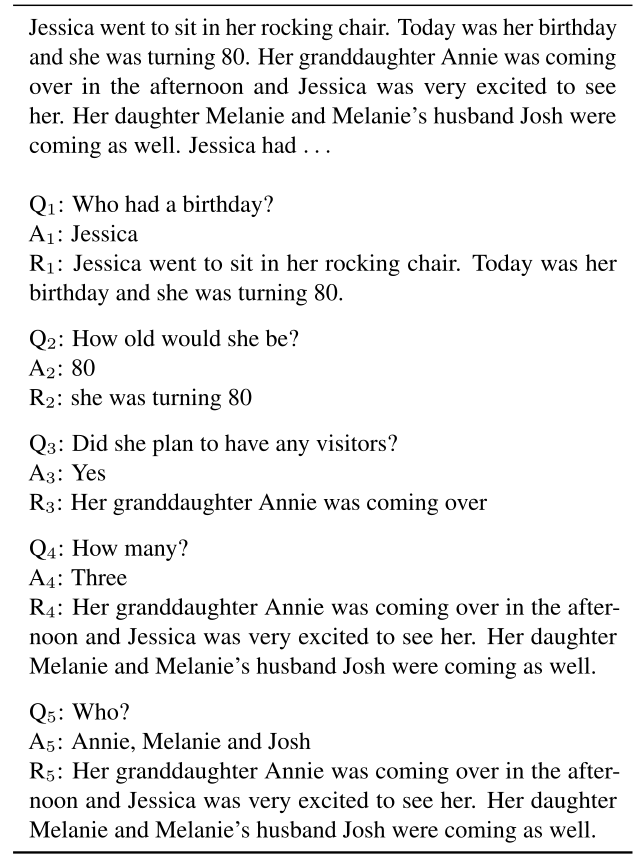
\includegraphics[width=8cm,height=10cm]{coqa.png}
%\end{figure}
\subsection{评估方法}
对于不同的MRC任务有不同的评估指标。
对于填空式任务与多项选择式任务都是属于客观题型,用准确率就可以衡量模型的性能。
例如对于测试集合中的所有问题$Q=\{Q_1,$$Q_2,\cdots,Q_m\}$,其中$m$代表问题的个数。如果模型预测出来的
$m$个答案中有$n$个是正确的,那么模型的准确率是$n/m$。

抽取式任务属于半客观题型,通常用精确匹配EM(Exact Match)和F1分数来评估模型。
EM评估指标可以看做是准确率的扩展,就抽取式任务来讲,EM要求
预测出来的所有单词要和标准答案
的所有单词要完全一致,EM值才为1,否则为0。
F1值的计算方式是一种模糊匹配,它是精确率和召回率
之间的调和平均数。精确率是指模型预测的答案中有多大比例的单词是标准答案中的单词。
召回率是指标准答案中的单词有多大比例在预测答案中出现。


对于自由答案式任务由于其答案形式不固定,一般采用单词水平的匹配率作为评分标准,常用标准用
ROUGE-L\upcite{Rouge}和BLEU\upcite{BLEU}。ROUGE-L用来计算标准答案和预测答案的最长公共子序列(Longest Common Subsequence,LCS),BLEU最初用于评估翻译性能,在应用到MRC任务上主要
用来衡量预测答案和真实答案之间的相似性。表5列举了本章介绍的所有数据集及相应的评估方法。


%\subsubsection{ROUGE}
%ROUGE\upcite{ROUGE}(Recall-Oriented Understudy for Gisting Evaluation)最初是用来
%评估生成文本摘要的一种方法,因为可以ROUGE的计算机制
%来评估MRC领域中自由答案型任务。ROUGE的评分有多种,在MRC领域较为常用的是ROUGE-L,
%ROUGE-L用来计算标准答案和预测答案的最长公共子序列(Longest Common Subsequence,LCS),
%ROUGE-L的计算
%公式如下:
%\begin{gather}
%    R_{LCS}=\displaystyle\frac{LCS(X,Y)}{m} \notag \\
%    P_{LCS}=\displaystyle\frac{LCS(X,Y)}{n} \\
%    F_{LCS}=\displaystyle\frac{{(1+\beta)}^2R_{LCS}P_{LCS}}{R_{LCS}+\beta^2P_{LCS}} \notag
%\end{gather}
%其中$LCS(X,Y)$表示标准答案与预测答案之间的最长公共子序列,
%$m$和$n$分别代表标准答案和预测答案中单词的个数,$\beta$是ROUGE-L的的参数,
%用来控制精确率和召回率的重要程度。

%\subsection{小结}
%本章介绍了MRC任务的定义以及根据答案类型的不同划分四种任务并且介绍了每一个任务的形式以及相关的数据集
%,同时简述了每一个任务下衡量模型性能所用的评估指标。
%下表5从数据集来源及规模,文章、问题以及答案的类型角度上对比了本章所介绍的所有数据集(其中QuAC和CoQA两个数据集细节见\ref{cmrc}节)。可以看到,MRC任务从最简单的填空型任务,逐步过渡到复杂的片段选择型任务,最后到更复杂的需要从多段落进行多步推理或者对话形式的任务。正是这些越来越具有挑战性的数据集的发布,极大的推动了MRC领域的发展。
\begin{table}[ht]
	\centering
	\caption{MRC常用数据集对比,Acc代表准确率 \\ Table 5 Comparison of common dataset in MRC}
	%\vspace{5pt}
	\resizebox{\textwidth}{!}{
		\begin{tabular}{l c c c c c c c}
			\toprule
			数据集&发布时间&文章来源/数量&文章类型&问题来源/数量&答案类型&评估指标 \\
			\midrule
			CNN\&Daily Mail\upcite{CNNDailyMail}&2015&新闻/$3\times 10^5$&单段落型&人工合成/$1.4\times 10^6$&填空式&Acc \\
			\midrule
			CBT\upcite{CBT}&2015&儿童读物/$108$&单段落型&人工合成/$6.8\times 10^5$&填空式&Acc \\
			\midrule
			CLOTH\upcite{CLOTH}&2016&英语考试&单段落型&英语考试/$1\times 10^5$&填空式&Acc \\
			\midrule
			MCTest\upcite{MCTest}&2013&儿童读物/$500$&单段落型&众包/$2\times 10^3$&多项选择式&Acc \\
			\midrule
			RACE\upcite{RACE}&2018&英语考试/$5\times 10^4$&单段落型&英语考试/$8.7\times 10^5$&多项选择式&Acc\\
			\midrule
			SQuAD\upcite{SQuAD1}&2016&维基百科/$536$&单段落型&众包/$1\times 10^5$&抽取式&EM/F1\\
			\midrule
			TriviaQA\upcite{TriviaQA}&2017&网页搜索/$6.6\times 10^5$&多段落型&搜索日志/$4\times 10^4$&抽取式&EM/F1\\
			\midrule
			SQuAD 2.0\upcite{SQuAD2}&2018&维基百科/$536$&单段落型&众包/$1.5\times 10^5$&抽取式&EM/F1\\
			\midrule
			NewsQA\upcite{NewsQA}&2017&新闻/$1\times 10^4$&单段落型&众包/$1\times 10^5$&抽取式&EM/F1\\
			\midrule
			HotpotQA\upcite{HotpotQA}&2018&维基百科&多段落型/&众包/$1.13\times 10^5$&抽取式&EM/F1\\
			\midrule
			WIKIHOP\upcite{WIKIHOP}&2018&维基百科&多段落型/&自动生成,需多步推理&抽取式&EM/F1 \\
			\midrule
			MS MARCO\upcite{MSmarco}&2016&搜素引擎/$2\times 10^5$&多段落型&搜索日志/$1\times 10^5$&自由答案式&ROUGE-L/BLEU\\
			\midrule
			DuReader\upcite{DuReader}&2018&搜索引擎/$1\times 10^6$&多段落型&搜索日志/$2\times 10^5$&自由答案式&ROUGE-L/BLEU\\
			\midrule
			NarrativeQA\upcite{NarrativeQA}&2017&小说和电影剧本/$1.5\times 10^3$&多段落型&众包/$4.6\times 10^4$&自由答案式&ROUGE-L/BLEU\\
%			\midrule
%			CoQA\upcite{CoQA}&2018&维基百科/127K&单段落型&提问者和回答者以对话形式生成问题和答案&自由答案型\\
%			\midrule
%			QuAC\upcite{QuAC}&2018&维基百科/100K&单段落型&类似于CoQA,不过文章对于提问者不可见&片段选择型\\
			\bottomrule
		\end{tabular}
	}
\end{table}





%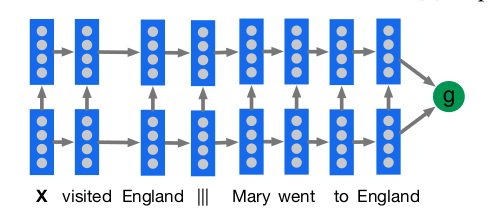
\includegraphics[]{Deep_lstm.png}

% \begin{table}
%     \caption{自动加表号}
%     \centering
%     \begin{tabular}{l l l}
%         \toprule
%         a&b&c
%         \midrule
%         value1&value2&value3
%         \bottomrule
        
%     \end{tabular}
% \end{table}




\begin{multicols}{2}
%\input{Introduction.tex}
\section{机器阅读理解任务概述}

%\footnotetext[1]{\url{www.cnn.com}}\label{1}\vspace{-10pt}
机器阅读理解(MRC)任务是为了使得计算机具有对自然语言文本理解的能力,像人类一样阅读并且理解一篇文章。
MRC可以用一个三元组$<D,Q,A>$来描述,其中$D$代表文章(Document)\footnote{本文中文章(Document)和段落(Passage)是同样的概念},$Q$表示问题(Question),$A$表示答案(Answer),即
给定一篇文章$D$和一些与文章$D$相关的问题$Q$,
要求模型通过阅读$D$之后给出$Q$的正确答案$A$,建模给定$D$和$Q$的条件下预测$A$的概率:$P(A|D,Q)$
。

MRC任务已经从早期的需要阅读一篇文章,答案是单个单词的阅读理解任务,发展到需要阅读多篇文章,并且答案需要从多篇文章中推理出来的阅读理解任务,使得阅读理解任务更加的贴近真实场景。
%甚至只需某个相关的上下文句子即可正确的填写出问题中的单词。经过近几年的MRC领域的快速发展,目前已经有很多数据集既需要模型从多篇文章中多步推理又要同时给出不限于文章中单词的答案,任务的难度显著上升。
本文按照Chen\upcite{base}
提出的分类方式,根据答案形式的不同将阅读理解任务概括为4类任务:填空式、多项选择式、抽取式和自由答案式。
%随着近年来MRC领域的发展出现了一些新兴的阅读理解任务如带有无答案问题的任务,对话形式的任务等,本文将机器阅读理解任务划分为yixia
下面对这四种类型任务分别进行叙述并介绍相关的数据集。



\subsection{填空式}
填空式阅读理解是指给定一篇文章$D$和一个与文章相关的问题$Q$,$Q$是通过删除
掉句子中某一个单词构成,要求模型根据$D$能够
正确的填写出$Q$缺失的单词$a$,且$a\in D$。填空型数据集的一个样例见表1。

典型的填空式数据集是由Google DeepMind和牛津大学发布于2015年的CNN\&Daily Mail\upcite{CNNDailyMail}数据集,
这是第一个较大规模的完形填空型阅读理解型数据集。从CNN\footnote{www.cnn.com\label{cnn}}中收集93k篇文章,从
Daily Mail\footnote{www.dailymail.co.uk\label{daily mail}}上收集220k篇文章。删去句子中的一个命名实体单词,
以此作为问题,构建了(文章-问题-答案)的三元组形式的语料库作为填空式的阅读理解任务。

相关的数据集还有
Hill等人\upcite{CBT}发布了(Children's Book Test,CBT)数据集,语料库来源于儿童读物(Gutenberg\footnote{https://www.gutenberg.org/\label{cbt}}工程)。与CNN\&Daily Mail的不同之处是删除的单词不局限于命名实体,还可能删除句子中的名词、动词和介词。
%每一篇文章是由20个连续的句子构成,删除第21个句子中的某个单词作为问题。
CLOTH\upcite{CLOTH}数据集是收集自中国中学生的英语考试试题中的完型填空题型。
%与之前的填空型数据集最大的不同是问题中删除的单词不像之前数据集的构建方式那样是由系统根据规则自动构建的,这样生成的问题往往没有目的性并且答案可能会出现歧义。
每一个问题是由专家为了测验学生英语水平而精心设计的,空白处位置的单词通常会考察学生的词汇、语法以及推理能力,因此CLOTH数据集相比于CNN\&Daily和CBT更具有挑战性。

%\begin{center}
\begin{table}[ht]
    %\centering
    %表格超出页边距用resizebox
    %\resizebox{\textwidth}{!}{
    \caption{CNN\&Daily Mail\upcite{CNNDailyMail}数据集的一个样例 \\ Table 1 An example of CNN\&Daily Mail dataset}
    %\vspace{5pt}

    \begin{tabular}{l p{15.0cm}<{\raggedright}}
        \toprule
        文章:&\tabincell{l}{What was supposed to be a fantasy sports car ride at Walt Disney World Speedway turned \\ 
                           deadly when a Lamborghini crashed into a guardrail. The crash took place Sunday at the \\ 
                           Exotic Driving Experience, which bills itself as a chance to drive your dream car on a race-\\ 
                           track. The Lamborghini’s passenger, 36-year-old Gary Terry of Davenport, Florida, died at \\ the
                           scene, Florida Highway Patrol said. The driver of the \textbf{Lamborghini}, 24-year-old Tavon \\ Watson
                            of Kissimmee, Florida, lost control of the vehicle, the Highway Patrol said. (...)} \\
        %\cmidrule(l){2-3}
        \midrule
        问题:&\tabincell{l}{Officials say the driver, 24-year-old Tavon Watson, lost control of a\_\_\_} \\
        %\cmidrule(l){2-3}
        \midrule
        答案:&Lamborghini \\
        \bottomrule
    \end{tabular}
    %}
    %\textbf{表1:CNN\& Daily Mail\upcite{Teaching Machines to Read and Comprehend}的一个样例}
\end{table}
%\end{center}

\subsection{多项选择式}
多项选择式这类任务是对于给定的文章$D$和问题$Q$以及多个
候选答案$A=\{A_1,A_2,\cdots,A_n\}$,
从$A$中选择正确的答案,建模概率:$P(A_i|D,Q)$,其中$A_i \in A$。
相关的数据集如MCTest\upcite{MCTest}和RACE\upcite{RACE}。多项选择型数据集的一个样例见表2。

MCTest是一个早期提出来的多项选择式数据集,问题形式为四选一。
%数据集收集自儿童故事语料库,类似这种基于故事文章的语料库
%构建数据集的还有上面提到的CBT\upcite{CBT}。
但是由于其规模比较小仅仅包含500篇故事文章很难利用神经网络模型来学习,因此MCTest通常用来作为验证集或测试集。

RACE\footnote{www.cs.cmu.edu/glail/data/race/\label{race}}数据集是从中
国中学生英语考试题中的阅读理解题型
建立的数据集。共有将近2.8万篇文章以及10万个问题,
%答案并不是简单的限制于
%文章中的单词,而且答案和问题中单词可能
%从没有在文章中出现过,利用单词匹配方式并不能达到很好的效果。
这些问题和候选答案都是由专家生成的,
%更加的接近真实世界的语义。
%RACE数据集中文章主题的覆盖度比其它的数据集更广泛,比如CNN\&Daily\upcite{CNNDailyMail}
%所有文章全都是来源于CNN新闻,SQuAD\upcite{SQuAD1}数据集所有的文章全都是来源于维基百科。
此外RACE数据集涵盖多个领域如新闻、故事、广告、传记等等,由于其类型的多样性因此可以更好的评估机器的阅读理解
能力。


\begin{table}[ht]
    %\centering
    %表格超出页边距用resizebox
    %\resizebox{\textwidth}{!}{
    \caption{RACE\upcite{RACE}数据集的一个样例 \\ Table 2 An example of RACE dataset}
    %\vspace{5pt}

    \begin{tabular}{l p{15.0cm}<{\raggedright}}
        \toprule
        文章:&\tabincell{l}{Runners in a relay race pass a stick in one direction. However, merchants passed silk, gold, \\ 
                           fruit, and glass along the Silk Road in more than one direction. They earned their living by \\ 
                           traveling the famous Silk Road. .. The Silk Road was made up of many routes, not one smo- \\oth 
                           path. They passed through what are now 18 countries. The routes crossed mountains and \\ deserts  
                           and had many dangers of hot sun, deep snow and even battles...}\\
        %\cmidrule(l){2-3}
        \midrule
        问题:&\tabincell{l}{The Silk Road became less important because\_\_\_} \\
        %\cmidrule(l){2-3}
        \midrule
        选项:& \tabincell{l}{A. it was made up of different routes \\
        B. silk trading became less popular \\
        \textbf{C. sea travel provided easier routes} \\
        D. people needed fewer foreign goods}\\
        %\cmidrule(l){2-3}
        \midrule
        答案:&C \\
        \bottomrule
    \end{tabular}
    %}
    %\textbf{表1:CNN\& Daily Mail\upcite{Teaching Machines to Read and Comprehend}的一个样例}
\end{table}

\subsection{抽取式}
抽取式阅读理解任务可以看做是填空式任务的扩展,不像填空式任务仅仅要求答案是原文中的某个单词,抽取式任务要求模型从原文中抽取一段连续的文本作为答案,且答案的长度不固定。
这类阅读理解任务是MRC领域较为流行的研究方向,主要原因在于从数据集的构建、评测指标以及应用价值等角度上看抽取式阅读理解是最合适的。
给出文章$D$和问题$Q$,问题的答案是$D$中的一段连续的单词构成。可以表示为$P(A|D,Q)$,其中$A=\{t_i,t_{i+1},\cdots,t_{i+k}\}(1\leq i\leq i+k\leq n)$,$n$代表$D$中
单词的个数,$k$代表答案的长度。抽取式阅读理解任务的样例见表3。
%抽取式阅读理解任务常用的数据集如SQuAD\upcite{SQuAD1}、
%NewsQA\upcite{NewsQA}、TriviaQA\upcite{TriviaQA}等。片段选择型的一个样例见表3。

SQuAD\upcite{SQuAD1}是抽取式阅读理解的代表性数据集,也是MRC领域最为
广泛使用的数据集之一,它的提出极大地推动了MRC领域的发展。
数据集由众包工人根据维基百科上面的文章给出问题,答案来源于文章中某段连续的文本,长度并不固定。
SQuAD含有536篇文章,总计十万多个问题-答案对
。类似的数据集如NewsQA\upcite{NewsQA},区别在于NewsQA文章来源于CNN新闻并且在NewsQA中某些问题
是没有答案的,这也使得后来Rajpurkar等人在SQuAD版本上又增加了五万个不可回答的问题构建了数据集SQuAD 2.0\upcite{SQuAD2}。
%对于这些带有不可回答问题的数据集,模型首先要清楚问题是否可以根据文章回答,在可回答的前提下给出答案,因此要求模型对文章的理解要更加的深刻。
%实验表明,那些在SQuAD数据集上效果很好的模型在SQuAD 2.0数据集上性能显著下降,这也说明了目前很多MRC模型都是基于浅层的语义匹配来寻找答案而不是真正的理解了文章。

之前的数据集都是给定文章后,由人工构造出与文章相关的问题和答案,但是现实世界中人们通常是先提出问题
然后搜寻相关的文章再找到答案。基于这一思想,Joshi等人\upcite{TriviaQA}首先从trivia上收集大量的问题-答案对,然后为每一个问题从网页上或者维基百科上搜索出相关的文章,这些文章就是答案的依据。最后构建出包含65万多个(问题-答案-文章)三元组的抽取式阅读理解数据集TriviaQA,这种由问题找文章的数据集构造方式使得问题和文章在句法和词汇上都有着较大的差异性,
这使得数据集难度更高。

目前大部分的抽取式数据集对模型的推理能力要求不高,主要原因在于回答这些数据集的问题往往只需要集中于某个句子的上下文或者在一篇段落上推理即可。为了提高模型的多步推理能力,
Yang等人\upcite{HotpotQA}发布了HotpotQA数据集,每一个问题对应多个段落,问题的答案往往需要在多个段落上逐步推理才能获得,同时要求模型预测回答问题所必须的线索句子(supporting facts)。
类似的数据集还有WIKIHOP\upcite{WIKIHOP},每一个样本来源于知识库中的三元组,要求模型从多篇维基百科文章中推理然后从多个候选中选出正确的答案。

\begin{table}[ht]
    %\centering
    %表格超出页边距用resizebox
    %\resizebox{\textwidth}{!}{
    \caption{SQuAD 1.1\upcite{SQuAD1}数据集的一个样例 \\ Table 3 An example of SQuAD 1.1 dataset}
    %\vspace{5pt}

    \begin{tabular}{l p{15.0cm}<{\raggedright}}
        \toprule
        文章:&\tabincell{l}{In 1870, Tesla moved to Karlovac, to \textbf{attend school at the Higher Real Gymnasium},\\ where
                            he was profoundly influenced by a math teacher Martin Sekulić. The classes were held\\ in German, 
                            as it was a school within the Austro-Hungarian Military Frontier. Tesla was able \\to perform int
                            egral calculus in his head, which prompted his teachers to believe that he was\\ cheating. He fini- shed a four-year term in three years, graduating in 1873. \\} \\
        %\cmidrule(l){2-3}
        \midrule
        问题:&Why did Tesla go to Karlovac? \\
        %\cmidrule(l){2-3}
        \midrule
        答案:&attend school at the Higher Real Gymnasium \\
        \bottomrule
    \end{tabular}
    %}
    %\textbf{表1:CNN\& Daily Mail\upcite{Teaching Machines to Read and Comprehend}的一个样例}
\end{table}
%\begin{multicols}{2}
\subsection{自由答案式}
抽取式任务这种从原文中抽取一段文本作为答案的约束并不能回答所有问题需要的答案,而且从文章中概括提炼出问题的答案也是更加的符合人们的阅读方式的。于是研究人员开始转向
自由答案式阅读理解任务,
这类任务的答案是自由形式的
,不局限于文章中的某些单词,语法上往往是更加的灵活。
可以表示为$P(A|D,Q)$,其中$A\subseteq D$或$A\nsubseteq D$。
%基于这些原因,自由回答式问答的数据集
%也因此公布出来并且受到广泛的关注,
%相关的数据集如MS MARCO\upcite{MSmarco}、DuReader\upcite{DuReader}和NarrativeQA\upcite{NarrativeQA},
自由答案式任务的一个样例见表4。

MS MARCO\upcite{MSmarco}是自由答案式阅读理解数据集的代表之一,由微软通过在必应搜索引擎的日志上收集用户
提出的问题,段落是来源于必应搜索引擎的返回的10个最相关的
查询段落,人工的从这些选择出来的段落中概括提炼出答案。
%然后由标注人员从这10个文本段落中找出那些与这个问题有关的文本段落,
%同时对于选出来的段落要标记为$\text{is\_select=1}$,表示这个段落和答
%案相关,从而可
%以训练模型。
如果不能从给出的10个段落中推理出答案,
那么这个问题就标记为无答案的问题。
%同样要保留在数据集中,目的就是让模型能够判别出问题是否可以回答。
DuReader\upcite{DuReader}是与MS MARCO类似的一个中文机器阅读理解数据集,类似于MS MARCO数据集的构造方式,问题和文章取自百度搜索和百度知道。

%答案同样是人工生成的,一个问题会给出5个相应的文本段落,很多问题需要推理多篇文章段落才能得到答案,甚至一些问题存在多个答案。
%MS MARCO和DuReader数据集的问题都是收集自搜索引擎中用户提出的问题,因此这两个数据集也更加的贴近真实场景。

%Kovcisky等人认为现在MRC领域大部分数据集的问题过于肤浅,而且答案往往只关注上下文信息,因此很多问题仅仅通过浅层的模式匹配
%就可以找到答案,他们发布的NarrativeQA数据集,收集自小说和电影剧本,要求模型在理解整部小说或剧本的前提下才能回答问题,要求模型需要有更强的理解能力和推理能力。


%\vspace{15\baselineskip}

\begin{table}[ht]
    %\centering
    %表格超出页边距用resizebox
    %\resizebox{\textwidth}{!}{
    \caption{MS MARCO\upcite{MSmarco}数据集的一个样例 \\ Table 4 An example of MS MARCO dataset}
    %\vspace{5pt}
	\centering%p{15.5cm}<{\raggedright}
    \begin{tabular}{l p{15.0cm}<{\raggedright}}
        \toprule
        文章1:&\tabincell{l}{Rachel Carson’s essay on The Obligation to Endure,is a very convincing argument about the \\
        harmful uses of chemical, pesticides, herbicides and fertilizers
        on the environment.} \\

        $.......$ \\
        文章5:&\tabincell{l}{Carson believes that as man tries to eliminate unwanted insects and weeds; however he is 
        act-\\ually causing more problems by polluting the environmen with, 
        for example, DDT and harm-\\ing living things}\\
        %\cmidrule(l){2-3}
        $.......$ \\
        文章10:&\tabincell{l}{Carson subtly defers her writing in just the right
        writing for it to not be subject to an induc-\\tion run
        rampant style which grabs the readers interest without
        biasing the whole article.}\\
        \hline
        问题:&Why did Rachel Carson write an obligation to endure? \\
        %\cmidrule(l){2-3}
        \midrule
        答案:&\tabincell{l}{Rachel Carson writes The Obligation to Endure
        because believes that 
        as man tries to elimin-\\ate 
        unwanted insects and weeds; however he is actually
        causing more problems by polluting \\ the environment.} \\
        \bottomrule
    \end{tabular}
    %}
    %\textbf{表1:CNN\& Daily Mail\upcite{Teaching Machines to Read and Comprehend}的一个样例}
\end{table}

%\subsection{对话型问答}
%虽然本节介绍的对话型任务按照答案形式上划分仍然可以划分到那四种类型里面,但是由于对话型问答任务与其它任务在数据集构造方式以及任务形式上有较大不同,因此本节单独列出对话型问答任务。
%除了按照答案形式上划分还可以根据文章类型划分,如单段落型阅读理解还是多段落型阅读理解。
%%
%%
%%根据问答形式划分,比如上面所介绍的所有数据集都属于单轮对话式问答,
%%即文章所对应的多个问题之间没有联系,每一个问题都是互相独立的。这并不符合
%%现实世界中人与人之间的对话交流,人们是通过多轮对话形式来交流的,每一轮的问题和答案都会影响后面的问答情况。
%然而无论是单段落型阅读理解还是多段落型阅读理解,它们都属于单轮对话问答,即问答的形式只有一轮,后面的问题与前面的问题和答案无关,每一个问题都是互相独立的。
%而在现实世界中人们是通过多轮对话形式来交流的,每一轮的问题和答案都会影响后面的问答情况。
%所以对话型任务来讲,在回答当前轮的问题时不仅需要考虑文章还需要考虑前几轮的问题和答案。
%具体可以表示为:给定$Q_i,D,{Q_{i-1},\cdots,Q_{i-k}},{A_{i-1},\cdots,A_{i-k}}$要求模型给出$A_{i}$。其中$Q_i,A_i$表示第$i$轮的问题和答案,$D$表示文章,$Q_{i-1},\cdots,Q_{i-k}$和$A_{i-1},\cdots,A_{i-k}$分别表示前$k$轮的问题和答案。即建模概率:
%\begin{equation}
%P(A_i|D,Q_i,Q_{i-1},\cdots,Q_{i-k},A_{i-1},\cdots,A_{i-k})
%\end{equation}
%
%目前典型的对话型问答数据集有CoQA\cite{CoQA}以及QuAC\cite{QuAC}。
%不同之处在于CoQA数据集的答案形式较为简单,类似于SQuAD 1.1\cite{SQuAD1},但是包含有yes/no以及unknown问题,其中unknown代表不可回答问题,此外还有一定比例的问题是自由答案形式。而QuAC数据集的构造过程中提问者没有看过文章而仅仅了解文章的标题,由回答者根据文章的内容选择出文章的一段文本作为答案,这种数据集构造形式类似于用户在搜素引擎中输入问题查找答案,目的是减少问题和文本之间的依赖,使得模型尽量避免通过浅层的匹配方式获得答案。
%对话型阅读理解数据集的一个样例见表5.其中每一个$R_i$代表答案依据,提供给模型训练。
%
%\begin{table}
%	\centering
%	\caption{对话型问答的一个样例,取自CoQA\cite{CoQA}}
%	\vspace{10pt}
%	\resizebox{\textwidth}{!}{\begin{tabular}{l p{15.5cm}<{\raggedright}}
%			\toprule
%			\multirow{3}{*}{文章}&Jessica went to sit in her rocking chair. Today was her birthday and she was turning 80. Her granddaughter Annie was coming over in the afternoon and Jessica was very excited to see her. Her daughter Melanie and Melanie's husband Josh were coming as well.\\
%			\cmidrule{2-2}
%			\multirow{3}{*}{第一轮}&$Q_1$: Who had a birthday? \\
%			&$A_1$: Jessica \\
%			&$R_1$: Jessica went to sit in her rocking chair. Today was her birthday and she was turning 80. \\
%			\cmidrule{2-2}
%			\multirow{3}{*}{第二轮}&$Q_2$: How old would \textbf{she} be? \\
%			&$A_2$: 80 \\
%			&$R_2$: she was turning 80. \\
%			\cmidrule{2-2}
%			\multirow{3}{*}{第三轮}&$Q_3$: Did \textbf{she} plan to have any visitors? \\
%			&$A_3$: Yes \\
%			&$R_3$: Her granddaughter Annie was coming over \\
%			\cmidrule{2-2}
%			\multirow{3}{*}{第四轮}&$Q_4$: \textbf{How many?} \\
%			&$A_4$: Three \\
%			&$R_4$: Her granddaughter Annie was coming over in the afternoon and Jessica was very excited to see her. Her daughter Melanie and Melanie's husband Josh were coming as well. \\
%			\cmidrule{2-2}
%			\multirow{3}{*}{第五轮}&$Q_5$: \textbf{Who?} \\
%			&$A_5$: Annie, Melanie and Josh \\
%			&$R_5$: Her granddaughter Annie was coming over in the afternoon and Jessica was very excited to see her. Her daughter Melanie and Melanie's husband Josh were coming as well. \\
%			\toprule  
%	\end{tabular}}
%\end{table}

%\begin{figure}[ht]
%	\centering
%	\caption{CoQA\upcite{CoQA}数据集的一个样例}
%	\vspace{10pt}
%	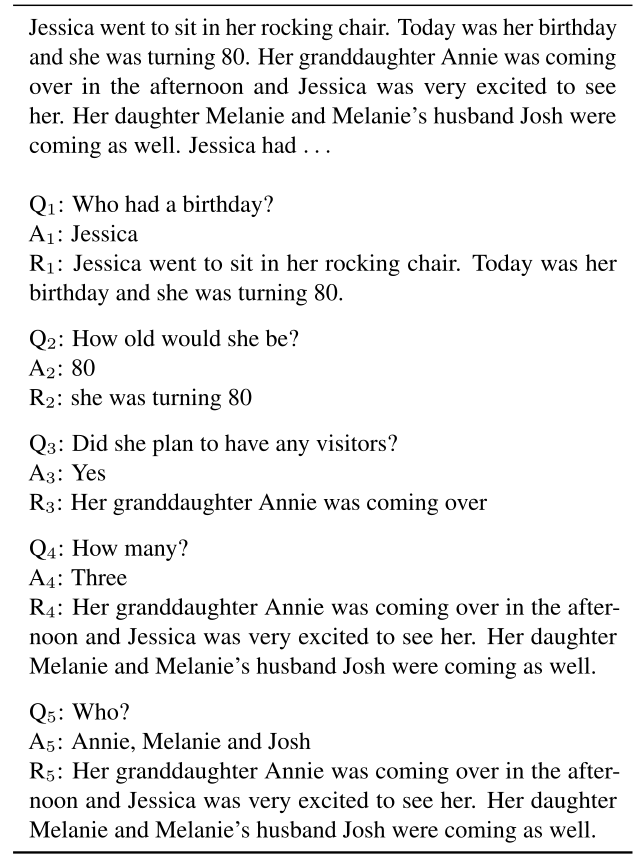
\includegraphics[width=8cm,height=10cm]{coqa.png}
%\end{figure}
\subsection{评估方法}
对于不同的MRC任务有不同的评估指标。
对于填空式任务与多项选择式任务都是属于客观题型,用准确率就可以衡量模型的性能。
例如对于测试集合中的所有问题$Q=\{Q_1,$$Q_2,\cdots,Q_m\}$,其中$m$代表问题的个数。如果模型预测出来的
$m$个答案中有$n$个是正确的,那么模型的准确率是$n/m$。

抽取式任务属于半客观题型,通常用精确匹配EM(Exact Match)和F1分数来评估模型。
EM评估指标可以看做是准确率的扩展,就抽取式任务来讲,EM要求
预测出来的所有单词要和标准答案
的所有单词要完全一致,EM值才为1,否则为0。
F1值的计算方式是一种模糊匹配,它是精确率和召回率
之间的调和平均数。精确率是指模型预测的答案中有多大比例的单词是标准答案中的单词。
召回率是指标准答案中的单词有多大比例在预测答案中出现。


对于自由答案式任务由于其答案形式不固定,一般采用单词水平的匹配率作为评分标准,常用标准用
ROUGE-L\upcite{Rouge}和BLEU\upcite{BLEU}。ROUGE-L用来计算标准答案和预测答案的最长公共子序列(Longest Common Subsequence,LCS),BLEU最初用于评估翻译性能,在应用到MRC任务上主要
用来衡量预测答案和真实答案之间的相似性。表5列举了本章介绍的所有数据集及相应的评估方法。


%\subsubsection{ROUGE}
%ROUGE\upcite{ROUGE}(Recall-Oriented Understudy for Gisting Evaluation)最初是用来
%评估生成文本摘要的一种方法,因为可以ROUGE的计算机制
%来评估MRC领域中自由答案型任务。ROUGE的评分有多种,在MRC领域较为常用的是ROUGE-L,
%ROUGE-L用来计算标准答案和预测答案的最长公共子序列(Longest Common Subsequence,LCS),
%ROUGE-L的计算
%公式如下:
%\begin{gather}
%    R_{LCS}=\displaystyle\frac{LCS(X,Y)}{m} \notag \\
%    P_{LCS}=\displaystyle\frac{LCS(X,Y)}{n} \\
%    F_{LCS}=\displaystyle\frac{{(1+\beta)}^2R_{LCS}P_{LCS}}{R_{LCS}+\beta^2P_{LCS}} \notag
%\end{gather}
%其中$LCS(X,Y)$表示标准答案与预测答案之间的最长公共子序列,
%$m$和$n$分别代表标准答案和预测答案中单词的个数,$\beta$是ROUGE-L的的参数,
%用来控制精确率和召回率的重要程度。

%\subsection{小结}
%本章介绍了MRC任务的定义以及根据答案类型的不同划分四种任务并且介绍了每一个任务的形式以及相关的数据集
%,同时简述了每一个任务下衡量模型性能所用的评估指标。
%下表5从数据集来源及规模,文章、问题以及答案的类型角度上对比了本章所介绍的所有数据集(其中QuAC和CoQA两个数据集细节见\ref{cmrc}节)。可以看到,MRC任务从最简单的填空型任务,逐步过渡到复杂的片段选择型任务,最后到更复杂的需要从多段落进行多步推理或者对话形式的任务。正是这些越来越具有挑战性的数据集的发布,极大的推动了MRC领域的发展。
\begin{table}[ht]
	\centering
	\caption{MRC常用数据集对比,Acc代表准确率 \\ Table 5 Comparison of common dataset in MRC}
	%\vspace{5pt}
	\resizebox{\textwidth}{!}{
		\begin{tabular}{l c c c c c c c}
			\toprule
			数据集&发布时间&文章来源/数量&文章类型&问题来源/数量&答案类型&评估指标 \\
			\midrule
			CNN\&Daily Mail\upcite{CNNDailyMail}&2015&新闻/$3\times 10^5$&单段落型&人工合成/$1.4\times 10^6$&填空式&Acc \\
			\midrule
			CBT\upcite{CBT}&2015&儿童读物/$108$&单段落型&人工合成/$6.8\times 10^5$&填空式&Acc \\
			\midrule
			CLOTH\upcite{CLOTH}&2016&英语考试&单段落型&英语考试/$1\times 10^5$&填空式&Acc \\
			\midrule
			MCTest\upcite{MCTest}&2013&儿童读物/$500$&单段落型&众包/$2\times 10^3$&多项选择式&Acc \\
			\midrule
			RACE\upcite{RACE}&2018&英语考试/$5\times 10^4$&单段落型&英语考试/$8.7\times 10^5$&多项选择式&Acc\\
			\midrule
			SQuAD\upcite{SQuAD1}&2016&维基百科/$536$&单段落型&众包/$1\times 10^5$&抽取式&EM/F1\\
			\midrule
			TriviaQA\upcite{TriviaQA}&2017&网页搜索/$6.6\times 10^5$&多段落型&搜索日志/$4\times 10^4$&抽取式&EM/F1\\
			\midrule
			SQuAD 2.0\upcite{SQuAD2}&2018&维基百科/$536$&单段落型&众包/$1.5\times 10^5$&抽取式&EM/F1\\
			\midrule
			NewsQA\upcite{NewsQA}&2017&新闻/$1\times 10^4$&单段落型&众包/$1\times 10^5$&抽取式&EM/F1\\
			\midrule
			HotpotQA\upcite{HotpotQA}&2018&维基百科&多段落型/&众包/$1.13\times 10^5$&抽取式&EM/F1\\
			\midrule
			WIKIHOP\upcite{WIKIHOP}&2018&维基百科&多段落型/&自动生成,需多步推理&抽取式&EM/F1 \\
			\midrule
			MS MARCO\upcite{MSmarco}&2016&搜素引擎/$2\times 10^5$&多段落型&搜索日志/$1\times 10^5$&自由答案式&ROUGE-L/BLEU\\
			\midrule
			DuReader\upcite{DuReader}&2018&搜索引擎/$1\times 10^6$&多段落型&搜索日志/$2\times 10^5$&自由答案式&ROUGE-L/BLEU\\
			\midrule
			NarrativeQA\upcite{NarrativeQA}&2017&小说和电影剧本/$1.5\times 10^3$&多段落型&众包/$4.6\times 10^4$&自由答案式&ROUGE-L/BLEU\\
%			\midrule
%			CoQA\upcite{CoQA}&2018&维基百科/127K&单段落型&提问者和回答者以对话形式生成问题和答案&自由答案型\\
%			\midrule
%			QuAC\upcite{QuAC}&2018&维基百科/100K&单段落型&类似于CoQA,不过文章对于提问者不可见&片段选择型\\
			\bottomrule
		\end{tabular}
	}
\end{table}




%\subsection{基于预训练模型的MRC模型}
% 使用预训练模型可以解决缺少标注数据的问题,因为预训练的模型已经在大量的无标签数据集上学习到了一些重要的特征等,因此应用到
% 具体任务时不需要大量的标注数据,也不需要长时间的训练即可达到很好的效果。
% 语言模型是NLP领域一个非常基础但同时也是非常
% 重要的一项任务,语言模型的目标就是根据一个单词的上下文预测出这个单词。
% 按照预测方式的不同可分为自回归语言模型和自编码语言模型,主要区别在于训练方式上是基于自回归形式还是自编码形式。
预训练模型近年来NLP领域获得了极大的关注度,基于预训练模型的方法在NLP几乎所有的任务上都要优于之前的模型。
预训练方式源自于迁移学习的概念: 首先在其它相关任务上预训练模型,使得模型已经学习到一些知识,然后在目标任务上做进一步优化,
实现模型所学知识的迁移。
对于NLP领域来讲,预训练过程就是在大量的文本数据上学习到通用的语言表示。在应用到下游任务时,预训练所学习到的知识提供了一个很好的
初始化点,从而加快模型的收敛并且提高模型的性能。此外预训练也对模型起到正则化的作用,使得模型避免在数据不充分的数据集上过拟合。

前面介绍的ELMo\upcite{ELMo}就是一个预训练模型,但是预训练的层次比较浅,对模型的提升效果也是有限的。
目前流行的几个预训练模型如,
GPT\upcite{GPT},BERT\upcite{BERT}以及基于BERT改进的预训练模型RoBERTa\upcite{RoBERTa},UNILM\upcite{UNILM},ALBERT\upcite{ALBERT}等,从MRC模型结构的角度看这些预训练模型相当于将上述模型通用结构的编码层和交互层融合在一起,在编码的同时进行段落与问题的交互,这些预训练模型刷新了MRC领域多个任务的最佳性能。
%全都是基于语言模型做预训练,因此也叫预训练语言模型。
%预训练的模型根据迁移方式的不同可以分为两种方式基于特征的方式(Feature-based)
%和基于微调的方式(Fine-tuning)。
%基于特征的方式是指对于预训练好的模型,应用到具体任务时固定模型的参数,将具体任务的数据通过预训练的模型得到数据的表示
%特征然后输入到根据具体任务设计的具体模型中。基于微调的方式是广泛采用的一种预训练模型的使用方式,具体的做法是在预训练模型的基础上加上少量的网络层,然后利用具体任务的
%标注数据训练整个网络模型。
%下面将主要概述NLP领域一些流行的预训练模型以及它们在MRC任务上的应用和效果对比。

\subsubsection{Transformer}\label{transformer}
鉴于目前几乎所有的预训练模型都采用transformer\upcite{Transformer}结构或者其变体作为模型的特征提取器,因此本节首先介绍transformer结构。
Transformer是由Vaswani等人提出了一种用于机器翻译的序列到序列(seq2seq)结构。
Encoder端由六个相同的层堆叠而成,每一层有两个子层,第一个子层采用多头(multi-head)自注意力机制,第二个子层采用前馈神经网络(Feed-Forward Network,FFN)构成。
之所以用自注意力机制是因为它既可以捕获句子中每一个单词的全局依赖关系而不受距离影响又可以并行计算。
对比公式(1),自注意力机制下$Q=K=V$,transformer中采用的计算方式如下:
\begin{equation}
\text{Attention}(Q,K,V)=\text{softmax}(\frac{QK^T}{\sqrt{d_k}})V
\end{equation}
其中$\sqrt{d_k}$代表张量维度。此外transformer采用的是多头(multi-head)自注意力机制,将$Q,K,V$三个张量线性映射成多份,每一份之间做注意力的运算最后拼接。
\begin{gather}
	\text{head}_i=\text{Attention}(QW_i^Q,KW_i^K,VW_i^V) \notag \\
	\text{Multi-head}(Q,K,V)=\text{concat}(\text{head}_1,\text{head}_2,\cdots,\text{head}_h)W^o
\end{gather}
其中$h$代表头的数目,是一个超参数,$W_i^Q,W_i^K,W_i^V,W^o$都是训练参数。

采用multi-head的目的是让模型联合关注序列中不同位置单词的不同表示子空间的信息,可以类比于卷积神经网络中利用多个卷积核做特征提取,目的同样是使得不同的卷积核关注的不同的特征。
此外
每一个子层都利用层正则化(layer normalization\upcite{layerNormal})和
残差连接(residual connection\upcite{RL})机制。
Decoder端与Encoder端类似,区别在于每一层额外添加了encoder-decoder注意力。

%Transformer的整体架构
%通过利用自注意力(self-attention)机制取代RNN那种序列式的计算方式,
%对于一个句子中的两个单词不考虑单词之间顺序的关系,直接计算它们之间的相关度,例如计算两个单词向量表示的内积。
%自注意力机制可以捕获句子中长距离依赖的特征关系,
%解决了循环神经网络固有的序列式传递信息导致后面的单词与前面的单词
%之间达不到有效的信息传递问题。
%通过自注意力机制不仅可以做到
%单词之间的全局交互同时其并行计算使得模型训练时间大幅减少。
Transformer的encoder端和decoder端都可以做特征提取器如BERT\upcite{BERT}用encoder端特征提取,GPT\upcite{GPT}用decoder端特征提取,实验证明在大规模数据集上transformer的特征提取能力要强于
基于RNN变体的编码器,目前几乎所有的NLP预训练模型都是利用transformer作为特征提取器。


\subsubsection{预训练模型}\label{pretrain}
%\subsubsection{相关预训练模型}
%ELMo\upcite{ELMo}是在2018年提出的一种预训练语言模型。
%传统的词嵌入模型如Word2Vec\upcite{word2vec},GloVe\upcite{GloVe}属于
%静态的词向量,训练好模型后一个单词的表示
%向量就是固定的,没有考虑上下文的信息,因此无法解决多义词问题。
%ELMo提出一个三层网络的模型
%,第一层就是词嵌入层用来提取单词特征,随后是两层BiLSTM网络分别提取
%单词的词性特征和语义特征。前向LSTM的目标是根据前$k-1$个词预测第$k$个词,从而计算出
%一个句子的概率,如公式(10)。反向LSTM的目标是根据最后的单词直到第$k+1$个单词预测第$k$个单词,
%具体如公式(11)。
%\begin{gather}
%    p(t_1,t_2,\cdots,t_N)=\prod_{k=1}^{N}p(t_k|t_1,t_2,\cdots,t_{k-1})\\
%    p(t_1,t_2,\cdots,t_N)=\prod_{k=1}^{N}p(t_k|t_{k+1},t_{k+2},\cdots,t_{N})
%\end{gather}
%最后的目标函数是最大化联合的前向和后向最大似然:
%\begin{equation}
%    \begin{split}
%    L(\Theta)&=\sum_{k=1}^{N}(\log p(t_1,\cdots,t_{k-1};\Theta)) \\
%        &+\log p(t_{k+1},\cdots,t_N;\Theta)
%    \end{split}
%\end{equation}
%在做阅读理解任务时,将文章和问题输入到模型中,每一层都会得到句子的语义表示,
%然后将每一层的特征加权求和作为ELMo的输出,此时得到的每一个单词的
%向量表示都是考虑了上下文的,将其作为下游模型嵌入层的输入。
%利用ELMo+BiDAF\upcite{BiDAF}
%结构超过之前单模型8.3个百分点。可以看出ELMo属于自回归语言模型,模型的迁移方式是基于特征的方式。




%\subsubsection{GPT}
OpenAI\upcite{GPT}提出一种生成式预训练模型(Generative Pre-Trained,GPT),使用多层的transformer\upcite{Transformer}的解码端作为特征提取器。模型采用两阶段的训练方式,先利用大规模无监督语料库训练前向语言模型,
然后在下游任务的少量监督数据集上微调模型,因此
GPT也是一种半监督学习方式,
%采用单向语言模型作为训练的任务,
预训练阶段的目标函数就是标准的单向语言模型的目标函数,见公式(1)。
%\begin{equation}
%    L(\Theta)=\sum_{k=1}^{N}(\log p(t_1,\cdots,t_{k-1};\Theta))
%\end{equation}
%GPT与ELMo的共同点是它们都属于自回归语言模型,
%而最大的不同之处在于迁移的设计上并不是像ELMo那种基于特征方式的迁移。GPT有统一的输入数据表示形式,
%而且在输入层并不需要继续设计复杂的网络模型而仅仅只需要简单的结构,在训练时整个网络模型的参数共同训练。
%这种基于微调的迁移方式被后续的其它预训练模型广泛采用。
%利用GPT在RACE\upcite{RACE}数据集上微调后达到的效果比之前最好的模型提高了5.7个百分点。
GPT是NLP领域首先提出的一种基于微调(fine-tune)的通用式网络结构,不仅仅在MRC领域,在很多其它的NLP领域都取得了很大的
进步。
%\end{multicols}
% \begin{center}
%     \textbf{表2 预训练语言模型对比}\\
%     \vspace{10pt}
%     \begin{tabular}{c c c c}
%         \toprule
%         模型&任务&模型结构&介绍 \\
%         \midrule
%         ELMo&单向LM&LSTM&拼接两个单向语言模型的语义信息,
                
%         基于特征形式迁移 \\
%         \midrule
%         GPT&单向LM&Transformer&首次采用预训练+微调形式
        
%         的两阶段任务,特征提取器采用transformer \\
%         \midrule
%         BERT&双向LM+NSP&Transformer&利用掩码语言模型和预测下一个句子共同作为训练任务 \\
%         \midrule
%         UNILM&单向LM+双向LM+Seq2SeqLM&Transformer&同时训练三种语言模型,采用掩码机制解决不同语言模型的约束问题 \\
%         \midrule
%         ALBERT&双向LM+SOP&Transformer&对比BERT采用矩阵分解和共享参数减少模型的参数量同时用句子顺序预测取代下一个句子预测 \\
%         \bottomrule
%     \end{tabular}
% \end{center}


%\subsubsection{BERT}
GPT属于自回归语言模型,自回归语言模型的缺点就是由于自回归的性质使得它不能同时利用一个单词的
上下文信息预测这个单词
Devlin等人\cite{BERT}提出BERT预训练模型,
与GPT最本质的不同在于预训练方式上采用的降噪自编码方式,
随机掩盖
掉一些单词,在输出层获得掩盖位置的概率分布,让模型根据掩盖位置的上下文预测这个单词,
这种机制也叫掩码语言模型(Masked Language Model,MLM)或双向语言模型。
%自回归语言模型的缺点就是由于自回归的性质使得它不能同时利用一个单词的
%上下文信息预测这个单词,
%ELMo虽然利用双向LSTM来预测单词但是这也只是两个单向的语言
%模型的拼接并不能当做双向语言模型。
%BERT在整个预训练的流程上采用GPT的方式,即预训练然后微调。
%但是BERT采用降噪自编码(DAE)的方式训练,具体的就是在输入数据中加入噪声,也就是随机掩盖
%掉一些单词,让模型根据掩盖掉单词的上下文预测这个单词,这种训练方式也叫掩码语言模型(MLM)。
%对比ELMo和GPT的目标函数,BERT的掩码语言模型的
MLM的目标函数为:
\begin{equation}
    \begin{split}
        L(\Theta)=\sum_{i=1}^{N}\log P(t_k|t_1,t_2,\cdots,t_{k-1},t_{k+1},\cdots,t_{N})
    \end{split}
\end{equation}
除了MLM任务外,还利用下一个句子预测(Next Sentence Prediction,NSP)任务使得模型
在诸如文本蕴含、问答这类需要判断两个句子关系的下游任务表现更好。
BERT的预训练过程实质上是
一个多任务学习的过程,通过MLM和NSP两个任务
提高了预训练模型的语义表达能力,其中MLM任务用来学习句子中词与词之间的语义关联而NSP任务用来学习两个句子之间的逻辑关系。
BERT在SQuAD\upcite{SQuAD1}数据集上的效果超过了人类的水平,在其它的NLP任务上也都有提升。
%\subsubsection{UNILM}

BERT开启了NLP领域预训练模型的时代,此后很多更加强大的预训练模型相继提出。这些预训练模型从结构上主要分为两大类:基于BERT的改进模型和XLNet。基于BERT的改进模型主要是针对BERT预训练阶段的两个任务MLM和NSP做改进,如
Liu等人\upcite{RoBERTa}提出RoBERTa模型,使用动态掩码替换BERT的静态掩码同时去除NSP任务;Li等人\upcite{UNILM}提出UNILM模型扩展了BERT预训练的任务,由于双向语言模型的性质使得BERT在生成任务上效果不好,
UNILM同时训练单向语
言模型(包括从左到右和从右到左)、双向语言模型以及Seq2Seq语言模型,使用掩码机制来解决不同的语言模型
约束问题;Lan等人\upcite{ALBERT}提出ALBERT模型,利用句子顺序预测(Sentence Order Prediction,SOP)任务改进了BERT的NSP任务;除了在预训练阶段改进训练任务外,Liu等人\upcite{MTDNN}提出MT-DNN模型在微调阶段引入了多任务学习机制,使用多个任务来微调模型参数使得模型具有更好的泛化型。

BERT模型以及基于BERT结构改进的模型在预训练阶段都采用降噪自编码的思想,所带来的问题就是预训练过程与微调过程不匹配,预训练使用的掩码机制在下游任务微调时不会被使用,导致两个过程存在数据分布的偏差。自回归语言模型虽然不存在这个问题,但是缺点是不能同时利用上下文信息。Yang等人\upcite{XLNet}提出的XLNet模型是一种可以同时获得上下文信息的自回归语言模型,
通过使用排列语言模型,引入双向自注意力流和循环机制兼顾了自回归和自编码语言模型的优点。

%
%BERT这种降噪自编码的方式虽然可以达到双向的利用上下文信息,但是由于其在预训练过程中对输入数据加入掩码而在微调时又不会加入掩码,导致
%了预训练过程与微调过程不匹配,存在一定的数据分布偏差,此外BERT对于屏蔽词的预测是独立的。基于上述问题,文献\cite{XLNet}提出一种新的
%预训练模型XLNet,它是一种可以获得双向的上下文信息的自回归语言模型,克服了传统的自回归语言模型和自编码语言模型各自的问题。XLNet采用的是
%排列语言模型(Permutation Language Model,PLM)
%,自回归模型中利用文本的前向或者后向序列的最大似然来建模,而PLM排列这个文本所有可能
%的序列顺序,仍然利用自回归语言模型的目标函数,但是综合所有可能的排列后每一个单词都可以获得双向的上下文信息。此外XLNet
%借鉴transformer-XL\upcite{Transformer-XL}中的片段循环机制引入循环机制可以捕获更长的句子依赖关系。

%文献\cite{RoBERTa}提出一种基于BERT改进其训练方式的预训练模型RoBERTa,其改进的方式包括:使用动态掩码替换静态掩码、去除NSP任务、使用更大的batch、
%更多的训练语料以及更长的训练时间。
%其中动态掩码是指对于输入数据中随机掩盖的单词并不是固定的,因为BERT的掩码机制是静态的,即对于每一个输入序列一旦选定了其中的
%的某个单词将其屏蔽,那么之后的整个训练过程该单词始终被掩盖。RoBERTa提出将输入数据复制10份,每一份都是随机掩盖部分单词,这样同一个输入序列
%就会有10种不同的掩码方式,从而达到动态掩码的目的。





%
%
%UNILM\cite{UNILM}扩展了BERT预训练的任务,由于双向语言模型的性质使得BERT在生成任务上效果不好,
%UNILM同时训练单向语
%言模型(包括从左到右和从右到左)、双向语言模型以及Seq2Seq语言模型,使用掩码机制来解决不同的语言模型
%约束问题。虽然是三个不同的语言模型作为训练任务但是共享同一个网络结构,也就是利用三个任务来联合的优化
%模型的参数。这种多任务学习的方式缓解了模型在某一个单一任务上容易出现过拟合的问题,
%使得预训练后的模型不仅在原有的自然语言理解任务上效果进一步提升,
%同时在自然语言生成任务上也达到了很好的效果。
%在微调阶段,对于自然语言理解任务(如文本分类、抽取式问答等)同BERT的微调方式一样,对于自然语言
%生成任务(如自动化摘要、生成式问答等)采用与预训练阶段Seq2Seq语言模型类似的方式在目标序列中
%随机的掩盖掉一些单词从而让模型根据源序列生成目标序列的单词达到生成任务的目的。
%UNILM不仅在抽取式QA数据集(如SQuAD)上超过BERT,在生成式QA数据集(如CoQA)上的表现远超过最初的基准模型。




%ALBERT\upcite{ALBERT}改进了BERT的NSP任务,BERT的NSP任务包含了两个子任务,来源于同一篇文章的两个连续的句子判别为正例,来源于不同文章的句子判别为负例,
%这使得模型不能集中于判断两个句子之间的顺序反而更加关注句子所表达的主题是否一致。因此ALBERT中用
%SOP(sentence-order prediction)取代NSP任务,SOP是指句子顺序预测,两个句子都是
%来源于同一篇文章的连续的句子,调换顺序后便是负例,这使得模型集中于预测句子之间的顺序关系,
%实验表明SOP任务使得模型的效果提升一个百分点。
%ALBERT的改进机制使得模型的预训练后的效果更好,在RACE\upcite{RACE},SQuAD 2.0\upcite{SQuAD2}等
%机器阅读理解数据集上的准确率超过BERT以及其它的预训练模型。
表11从预训练任务、模型采用的特征提取器等详细对比了本文介绍的所有预训练模型。表12对比了几个预训练模型在两个常用的MRC数据集上的表现。
% \subsection{小结}
% 传统的静态的预训练词向量虽然可以给模型性能带来一定程度的提升,但是这种提升非常有限。主要原因是
% 其静态的性质无法解决多义词的
% 问题而且所学习到的语义信息也是浅层的,仍然需要模型在标注数据集上从头学习。
% ELMo的出现使得静态词向量的问题得以解决,并且这种利用语言模型作为训练任务的方式也被后续的其它
% 预训练模型采用。GPT首次提出预训练过程结合微调过程的这种两阶段方式,使得不需要设计复杂的网络模型即可在
% 多个NLP任务上达到显著地提升。BERT是NLP预训练史上重要的里程碑模型,后续的其它更加优秀的
% 预训练模型如ALBERT、UNILM也都是在BERT的基础上进行进一步优化如:引入生成任务、改进训练方式等。

\begin{table}[ht]
	\caption{预训练模型对比\\ Table 11 Comparison of pre-trained model}
	\centering
	%\vspace{10pt}
	%表格超出页边距用resizebox
	\resizebox{\textwidth}{!}{
		\begin{tabular}{c c c c}
			\toprule
			模型&任务&模型结构&介绍 \\
			\midrule
			ELMo\upcite{ELMo}&\tabincell{c}{前向LM \\ 反向LM}&LSTM&\tabincell{c}{拼接两个单向语言模型的语义信息,\\ 基于特征形式迁移} \\
			\midrule
			GPT\upcite{GPT}&前向LM&Transformer&首次采用预训练+微调形式 \\
			\midrule
			BERT\upcite{BERT}&MLM+NSP&Transformer&利用掩码语言模型(MLM)和下一句预测(NSP)共同作为训练任务 \\
			\midrule
			MT-DNN\upcite{MTDNN}&MLM+NSP&Transformer&预训练过程与BERT一致,微调阶段采用多任务学习 \\
			\midrule
			XLNet\upcite{XLNet}&PLM&Transformer-XL&\tabincell{c}{采用排列语言模型(PLM),双向自注意力流\\模型以自回归方式训练但是基于上下文预测} \\
			\midrule
			RoBERTa\upcite{RoBERTa}&MLM&Transformer&采用动态掩码机制,去除NSP任务 \\
			\midrule
			UNILM\upcite{UNILM}&\tabincell{c}{前向LM+反向LM\\ +MLM\\ +Seq2SeqLM}&Transformer&\tabincell{c}{同时训练多种语言模型,\\ 采用掩码机制解决不同语言模型的约束问题} \\
			\midrule
			ALBERT\upcite{ALBERT}&MLM+SOP&Transformer&\tabincell{c}{对比BERT采用矩阵分解和共享参数减少模型的参数量,\\ 同时用句子顺序预测任务(SOP)取代下一个句子预测任务(NSP)} \\
			\bottomrule
		\end{tabular}
	}
\end{table}

 \begin{table}[ht]
     \centering
     \caption{预训练模型对比}
     \begin{tabular}{l c c}
         \toprule
         \multirow{2}{*}{模型}& SQuAD 2.0\upcite{SQuAD2} & RACE\upcite{RACE}\\
         \cmidrule(lr){2-2} \cmidrule(lr){3-3} 
         &EM/F1& Acc \\
         \midrule
         $\text{GPT}_{v1}$\upcite{GPT}&-&59.0\\
         \midrule
         $\text{BERT}_{large}$\upcite{BERT}& 80.0/83.1&72.0\\
         \midrule
         XLNet\upcite{XLNet}&86.4/89.1 &81.8\\
         \midrule
         RoBERTa\upcite{RoBERTa}&86.8/89.8 &83.2\\
         \midrule
         ALBERT\upcite{ALBERT}&88.1/90.9 &86.5\\
         \bottomrule
     \end{tabular}
 \end{table}


%\subsubsection{的MRC模型}
%在预训练模型出现后不仅仅在MRC任务上,在其它的NLP任务上模型的结构都发生了较大的变化,
%在模型的基础上利用具体任务的数据微调模型即可达到很好的效果。
%%但是预训练模型毕竟是一个通用式的模型,
%%它给了模型很好的初始化参数,不过要想达到更好的效果仍然要根据具体任务的形式来设计模型。
%下面列举几个MRC数据集上目前效果较好的基于预训练模型的MRC模型。
%
%人在做阅读理解问题的时候通常会先带着问题大致的浏览一下这篇文章,对这篇文章的含义有一个大致的了解。之后再根据问题详细的阅读文章寻找答案。受到这种阅读形式的启发,Zhang等人\upcite{Retrospective}提出一种回顾式阅读器(Retrospective Reader,Retro-Reader)模型。整个模型由两个步骤构成:(1)第一步先简要的略读文章,建模文章与问题的大致关联给出初步的判断该问题是否可以回答。(2)第二步是精读模块,目的是验证可回答性并且给出最终判断。模型的编码器采用强大的预训练模型ALBERT。Retro-Reader在SQuAD 2.0\upcite{SQuAD2}数据集上显著优于其它模型。
%
%%如何训练出一个性能更加强大的预训练模型成为近年来NLP领域的研究热点。
%Zhang等人\upcite{DCMN}
%利用BERT\upcite{BERT}和XLNet\upcite{XLNet}作为编码器同时采用文献\cite{Co-matching}提出的co-matching方法提出了DCMN模型,在RACE\upcite{RACE}
%数据集上达到了很高的准确率。
%而后在DCMN的基础上引入选项交互模块和段落选择模块提出DCMN+\upcite{DCMN+}模型,模型的性能进一步提升。
%
%BERT以及基于BERT改进的预训练模型其数据输入形式只能是两个句子的拼接因此并不适合直接处理CoQA这种对话型阅读理解数据集。
%%Qu等人\upcite{HAE}提出一种简单而有效的模型,仅仅需要在BERT模型的输入端为每一个单词添加两个额外的向量用来表明这个单词有没有在历史答案中出现过,文中称这两个向量为(History Answer Embedding,HAE)。实验表明BERT+HAE模型较之前的模型可以处理更多的历史对话信息。
%Zhu等人\upcite{SDNet}
%提出SDNet模型,以基于特征的方式迁移BERT作为编码器,同时将之前轮次的问题和答案拼接到当前轮的问题上构成一个新问题。模型采用自注意力机制获得历史对话信息之间的交互语义,具体的计算方式采用FusionNet\upcite{Fusionnet}模型提出的融合方法。
%Ohsugi等人\upcite{simpleqa}以基于微调的方式迁移BERT模型。
%将历史对话信息每一轮的问题与答案分别与文章连接送入
%BERT,将每一个BERT的输出连接作为输出层的输入。两个模型在CoQA\upcite{CoQA}和QuAC\upcite{QuAC}两个对话型数据集上的效果均超过前面的BiDAF++\upcite{Clark},FlowQA\upcite{FlowQA}等利用复杂交互机制的模型。
%由于预训练模型UNILM\upcite{UNILM}改进了BERT的训练任务,
%增加了自回归语言模型以及seq2seq语言模型使得其
%在生成式任务上的效果很好,在CoQA数据集上远远的超过于Reddy等\upcite{CoQA}提出的基准模型。




\subsubsection{迁移预训练模型}
预训练模型具有强大的文本表征能力,但是在应用到机器阅读理解任务上还需要根据具体的数据集特点设计不同的微调网络结构。以BERT系列的预训练模型为例,预训练阶段和微调阶段除了输出层外共享相同的体系结构,在做抽取式阅读理解任务时,输出层最简单的设计方式是仅利用两个向量与段落的向量表示计算答案在段落中起始位置和终止位置的概率。
对于其它形式的阅读理解任务,往往根据任务的特点在输入层和输出层设计相应的结构,相关的工作可以参照\upcite{HAE,simpleqa,Retrospective}。
另一种迁移预训练模型的方式是基于特征形式的迁移,将具体任务的数据送进预训练模型,预训练模型的特征表示作为下游模型的输入,训练时固定预训练模型的参数。


%预训练模型根据迁移方式的不同可以分为两种方式:(1)基于特征的方式(Feature-based)
%(2)基于微调的方式(Fine-tuning)。
%基于特征的方式是指将具体任务的数据送进预训练模型,将得到的文本表示
%特征输入下游模型结构中。
%
%基于微调的方式是广泛采用的一种预训练模型的使用方式,具体的做法是在预训练模型的基础上加上少量的网络层,然后利用具体任务的
%标注数据训练整个网络模型。



虽然设计一个强大的预训练模型具有更好的泛化型和应用价值,但是预训练模型所消耗的计算资源是巨大的,
因此如何利用预训练模型结合具体任务改进模型的结构是至关重要的。
% \begin{center}
%     \begin{tabular}{l c}
%         \toprule
%         单模型&EM/F1 \\
%         \midrule
%         MatchLSTM with Pointer Network& 64.7/73.7 \\
%         \midrule
%         Dynamic Coattention Network& 66.2/75.9 \\
%         \midrule
%         BiDAF&68.0/77.3 \\
%         \midrule
%         R-Net&72.3/80.7 \\
%         \midrule
%         QANet(data augmentation x3)& 76.2/84.6\\
%         \midrule
%         ELMo+BiDAF&78.6/85.8\\
%         \midrule
%         $\text{BERT}_{large}$(+TriviaQA)& 85.1/91.8 \\
%         \bottomrule
%     \end{tabular}
% \end{center}
% \begin{table*}[!hp]
%     \centering
%     \begin{tabular}{l c c c c}
%         \toprule
%         &SQuAD 1.1(F1)&SQuAD 2.0(F1)&RACE(Acc)&CoQA \\
%         \midrule
%         ELMo+BiDAF&85.8&-&-&- \\
%         GPT1&
%         \bottomrule
%     \end{tabular}
% \end{table*}

% \begin{table}
%     \begin{tabular}{l c}
%         \toprule
%         训练任务&目标函数 \\
%         \midrule
%         前向语言模型&$P(t_1,t_2,\cdots,t_N)=\prod_{k=1}^{N} P(t_k|t_1,t_2,\cdots,t_{k-1})$ \\
%         \midrule
%         反向语言模型&$P(t_1,t_2,\cdots,t_N)=\prod_{k=1}^{N} P(t_k|t_{k+1},t_{k+2},\cdots,t_N)$ \\
%         \midrule
%         掩码语言模型&$P(t_1,t_2,\cdots,t_N)=\prod_{k=1}^{N} P(t_k|t_1,t_2,\cdots,t_{k-1},t_{k+1},t_{k+2},\cdots,t_N)$ \\
%         \bottomrule
%     \end{tabular}
% \end{table}

% \subsubsection{迁移预训练模型}
% 训练好一个模型后应当考虑如何迁移这个预训练模型到具体的任务上。
% 按照迁移形式的不同可以分为(1)基于特征的迁移方式和(2)基于微调的迁移方式。
% % 基于特征的迁移方式是指将数据输入到预训练模型中然后提取出模型对输入数据的特征表示
% % ,将这组特征作为下游任务模型的输入,训练时预训练模型的参数是固定的。这种基于特征的迁移形式
% % 相当于把预训练模型当做语义编码器,上层仍需要设计具体的模型。

% % 基于微调的迁移方式是指将数据输入到预训练模型中,然后将预训练模型的输出作为
% ELMo\upcite{ELMo}是典型的基于特征的迁移方式,

% GPT\upcite{GPT}是典型的

\section{神经机器阅读理解模型}
随着大规模机器阅读理解数据集如CNN\&Daily Mail\upcite{Teaching Machines to Read and Comprehend},SQuAD 1.1\upcite{SQuAD1}等的发布以及
深度学习技术的发展,神经机器阅读理解模型的性能显著的超过传统的基于规则和特征的模型,随着NLP领域预训练模型的发展,基于预训练模型
来做MRC任务的模型性能再一次的提升。用于MRC任务的深度学习模型的整体框架主要包括如下几个层:词嵌入层、语义编码层、语义交互层、答案预测层。

1)词嵌入层:如何将文本有效的表示成计算机可以处理的形式同时可以有效地利用单词之间的语义一直的NLP领域
的重点问题。分布式表示是将单词用一个低维度的稠密向量表示,即将单词嵌入到一个低维稠密空间中,因此这种表示方式也叫词嵌入。
从早期的one-hot形式编码到词袋模型再到分布式表示技术最后到基于上下文的词嵌入技术,每一种技术的出现都证明了一个好的文本表示方法可以
极大地提升模型的性能。

2)语义编码层:这一层的目的是在词嵌入层的基础上通过对词嵌入层的输入文本做特征提取,进一步获得句子层面的语义信息。常用的特征提取器
有基于RNN的变体如LSTM\upcite{lstm}和GRU\cite{s}等。但由于梯度消失问题不能解决长距离依赖问题,使得其
特征提取能力始终受限。Transformer\upcite{Transformer}通过利用自注意力机制取代RNN那种序列式的计算方式,通过自注意力机制不仅可以做到
单词之间的全局交互同时其并行计算使得模型训练时间大幅减少。实验证明在大规模数据集上transformer的特征提取能力要强于
基于RNN的编码器,目前几乎所有的NLP预训练模型都是利用transformer作为特征提取器。

3)语义交互层:在预测答案时需要将问题的语义信息与文章的语义信息关联,这样模型在预测答案时才能知道文章中哪一部分是问题的答案。
通常利用注意力机制实现这一目标,注意力机制就是让模型关注到重点的部分,不同的注意力计算方式很大程度上的影响模型性能,
后面将详细介绍基于注意力机制的模型以及它们不同的计算方式。

4)答案预测层:这是整个模型架构的最后一层,用来输出预测的答案。如前面所提到的MRC任务大致分成四类,因此这一层的设计需要
考虑到答案形式。对于填空型任务,答案的输出是文章中的一个单词。对于多项选择任务,答案的输出是从多个候选答案中选择出正确的选项。
对于片段选择型任务,答案的输出是文章中某段连续的文本。对于自由答案型任务,答案的输出不限固定的文本,而是根据文章中的单词生成的答案。
此外还有不可回答的问题,此时模型的输出还要考虑到问题是否可以回答。

下面介绍神经机器阅读理解模型中基于注意力机制的模型和基于预训练模型的模型。
%\input{embedding_layer.tex}




% \subsection{基于注意力机制的模型}
交互层是整个网络模型中关键的一层,前面的编码层输出的是问题和文章中每个单词的上下文语义编码,每个单词
关注了自己所在句子的上下文单词,但是却并没有关注对应的句子。而我们在做阅读理解问题时,通常是带着
问题去文章中找答案,我们要知道文章中每一个单词和问题之间的相关度。因此交互层的目的就是让文章的语义信息与问题的
语义信息融合,以此达到对文章更深层次的理解,而交互层中最常用的方法就是注意力机制。

注意力机制简单的来说就是为序列的每一个位置生成一个权重值,这个值代表当前位置的单词对预测结果
的重要性。文献\cite{neural machine translation by jointly learning to align and translate}最早将
注意力机制应用在机器翻译领域,获得了极大的反响。这种注意力的思想就是在解码端每次生成一个单词
时要对编码端的句子做关注,也就是注意力的计算,具体的就是利用解码端的单词与编码端序列计算出一个权值分布,这个权值表示的
是编码端每一个单词对解码端单词的重要程度,然后利用权值分布对编码端序列加权求和得到一个固定长度的向量,这个向量就是注意力的计算结果
,并且作为下一个单词输入的一部分,这属于一种动态式的计算方式。
而这种
在将注意力计算结果送入到循环神经网络中并且对于循环神经网络的
隐藏状态同时参与注意力计算的网络也叫基于注意力的循环神经网络。
以下将首先介绍MRC任务中注意力机制之间的差异,然后分析各个模型将注意力机制应用在MRC任务上以及它们之间的区别与联系。

\subsubsection{MRC中的注意力}
% 单方向注意力的运算机制类比于人类做阅读问题的过程: 带着问题到文章中找答案,从文章的角度
% 对问题进行总结,获得文章对问题的注意力。
% 也就是先看问题,然后对于文本段落中各个部分生成一个注意力权重,代表这个部分与问题的相关程度,
% 利用注意力权重对文本的各个部分加权求和就可以得到文本段落与问题之间的相关性信息。
不同于机器翻译任务,只能将encoder端的单词语义信息融入到decoder端。
在机器阅读理解问题上,文章和问题都可以作为encoder或者decoder。这种情况下做注意力运算有两个方向,即从问题到文章,从文章到问题这两个方向。从问题到文章的注意力是指利用注意力权值
对文章的语义表示加权求和,将文章的语义信息融合到问题上。从文章到问题注意力是指将问题的语义信息融合到文章中,即文章的每一个单词都会
关注问题。
以问题到文章的注意力计算过程为例,$P=[p_1,p_2,\cdots,p_n]$代表文章的语义信息,其中的每一个
$p_i$代表文章中单词的语义向量表示,$Q$代表整个问题的语义信息。问题到文章的注意力就是利用问题
的语义信息和文章中每一个单词的向量表示计算它们之间的相关性,最后得到一组注意力权重$\alpha=[\alpha_1,\alpha_2,\cdots,\alpha_n]$
表示文章与问题之间的相关程度,利用$\alpha$对文章加权求和就可以提取出来文章中与问题最相关的单词,
这些单词对于回答问题是至关重要的。
具体计算过程如下:
\begin{gather}
    \alpha_i=\text{softmax}(s(p_i,Q)) \notag \\
    C=\sum_{i=1}^{n}\alpha_ip_i
\end{gather}
其中$s(p_i,Q)$就是计算问题
的语义信息和文章中每一个单词的向量表示它们之间的相关性的一个函数,常用的计算方式有点积、双线性项、
加法模型,分别见如下公式:
\begin{gather}
    s(p_i,Q)=p_i^TQ \\
    s(p_i,Q)=p_i^TWQ \\
    s(p_i,Q)=v^T\tanh(Wp_i+UQ)
\end{gather}
上面的式子是将问题压缩成一个固定维度的向量,得到的注意力权重也是一维的,因此也成为一维注意力,与其相对应的是二维注意力,即对于问题中的
每一个单词都会和文章做注意力计算,得到的注意力权重是二维向量。

如果按照注意力的计算形式上区分,
又可以分为one-hop和multi-hop形式。one-hop,也叫“单跳结构”是指仅仅通过一次计算得到注意力权值然后加权求和得到注意力结果,这也是一种
静态的计算形式。与之对应的是multi-hop,也叫“多跳结构”。one-hop形式下仅仅只做一次交互计算,而注意力机制虽然可以提取相关的重要信息,但是
它仍然是基于浅层语义信息的相似度计算。在机器阅读理解任务中,对于复杂的问题通常是不能在一个句子中找出答案,需要多步推理才能寻找答案,如下图中
的例子
% \begin{figure*}
%     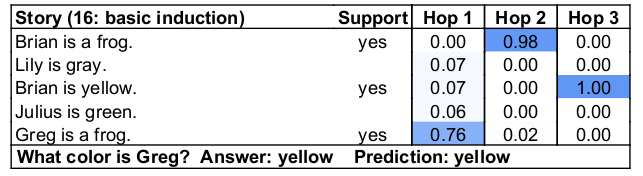
\includegraphics[]{multihop.png}
% \end{figure*}
%当前时刻计算的注意力结果要保留到下一时刻,即每一时刻都要计算注意力,是一种动态的计算形式,典型的代表是Bahdanau注意力\cite{neural machine translation by jointly learning to align and translate}。
我们可以看到想要得到最终的答案需要进行三次推理过程,在每一个推理过程中都会变换注意力关注的对象。
实现多步推理这种机制通常有三种方式:
1)基于之前时间步所计算得到的关注问题的文章语义信息计算下一时间步的文档和问题交互,如Impatient Reader\upcite{Teaching Machines to Read and Comprehend}。
2)利用RNNs这种基于上一时刻隐藏状态更新下一时刻隐藏状态的循环特性来达到多步推理,如Match-LSTM\upcite{Machine comprehension using match-lstm and answer poi
nter}。
3)引入额外的记忆单元存储语义信息,目的是希望解决RNN中不能够长期依赖导致信息丢失的问题,典型的如文献\cite{memory networks}
提出的记忆网络(memory networks)。

此外还有自注意力机制,自注意力机制是文本的向量表示和自身做交互,即文本中所有单词之间都会计算注意力,与单词的
位置顺序无关,这样对于两个距离较远的单词仍然可以交互,
循环神经网络这种序列式的计算机制非常适合处理文本句子这种序列式数据,但是也正因如此,网络的训练
是非常耗时的同时存在梯度消失的问题使得模型不能捕获长距离单词之间的关联信息。
自注意力机制(self attention)主要的思想就是撇弃这种序列式的计算方式,对于一个句子
中的两个单词不考虑单词之间顺序的关系,直接计算它们之间的相关度,例如计算两个单词向量表示的内积。
Self attention可以捕获句子中长距离依赖的特征关系,而且这种计算方式是并行的,极大地加快了模型的训练速度。
解决了循环神经网络固有的序列式传递信息导致后面的单词与前面的单词
之间达不到有效的信息传递问题。

下表详细的列举了本文介绍的所有模型的注意力机制。

\begin{center}
    %\textbf{}
    \resizebox{\linewidth}{!}{
        \begin{tabular}{c c c c}
            \toprule
            模型&注意力方向&注意力维度&推理模式 \\
            \midrule
            Attentive Reader\upcite{Teaching Machines to Read and Comprehend}&问题到文章&一维注意力&单跳结构 \\
            \midrule
            Impatient Reader\upcite{Teaching Machines to Read and Comprehend}&问题到文章&二维注意力&多跳结构 \\
            \midrule
            Standford Reader\upcite{AR}&问题到文章&一维注意力&单跳结构 \\
            \midrule
            AS Reader\upcite{ASR}&问题到文章&一维注意力&单跳结构 \\
            \midrule
            IA Reader\upcite{IAReader}&问题到文章&一维注意力&多跳结构 \\
            \midrule
            GA Reader\upcite{GAReader}&文章到问题&一维注意力&多跳结构 \\
            \bottomrule
        \end{tabular}
        }
\end{center}




\subsubsection{相关模型}

%\subsubsection{Attentive Reader and Impatient Reader}
文献\cite{Teaching Machines to Read and Comprehend}最早利用神经网络模型并且融入注意力机制做MRC任务。
文中提出两种不同的单向注意力机制Attentive Reader
和Impatient Reader,均是计算问题到文章的注意力。
Attentive Reader是将问题表示为一个固定长度的向量然后与文章中每一个单词做注意力计算,然后利用注意力权重对文章
中的单词的向量表示加权求和得到一个固定长度的
向量即为注意力运算后的结果,然后与问题联合预测答案,可见这种注意力的计算方式仅仅只计算一次,因此也叫one-hop。
这种方式类似于人在阅读时带着问题去文章中找答案。
Impatient Reader计算注意力的机制类似于文献\cite{neural machine translation by jointly learning to align and translate}
的方式,也属于一种multi-hop的计算。并不是将
问题表示为一个固定长度的向量,而是对于问题中的每一个单词都要和整个文章做注意力计算,而且计算的结果
要和下一个单词以及文章共同做注意力计算,最后一个单词的注意力结果作为整个Impatient Reader计算注意力过程的结果。
这种方式类似于人在阅读过程中不断的在问题和文章之间做关注。
文献\cite{AR}在Attentive Reader的基础上利用双线性项(公式8)取代原有的利用tanh函数的加法模型(公式9)并且直接将
对文章加权求和后得到的向量作为预测答案的输入而不是联合问题$Q$的语义信息,实验证明这种简化反而提高了模型的准确度。

文献\cite{memory network}提出的记忆网络并不能端到端的训练。为了处理这个问题,文献\cite{MemN2N}提出一种端到端的记忆网络(MemN2N)。
利用记忆槽存储文档中每一个句子的嵌入矩阵,记忆槽的状态以及问题的语义信息会随着与文档的多次交互不断更新。

文献\cite{IAReader}提出Iterative Attention Reader(IA Reader)模型,利用BiGRU\upcite{BiGRU}存储每一次
迭代计算得到的问题和文章的交互信息。在每一时间步上,首先利用上一次的BiGRU的状态与问题做一维注意力匹配提取出问题的语义信息,
然后再结合上一次的BiGRU的状态与文章再做一维注意力匹配从而提取出文章的语义信息。将问题与文章的语义信息
通过各自的门控单元作为BiGRU当前时刻的输入,其中门控单元采用前馈神经网络用来解决当前时间步下问题和文章的语义信息提取不充分的问题。

文献\cite{GAReader}提出Gated Attention Reader(GA Reader)模型,类似于IA Reader\upcite{IAReader}模型同样采用
BiGRU作为编码模块实现多跳结构。在每一步的推理过程中,首先通过BiGRU得到问题的语义信息然后对文章的
每一个单词做注意力的计算,同时采用点乘计算的门控机制建模
当前时间步的推理过程下关注了文章第$i$个单词的问题语义信息与文章第$i$个单词的语义信息影响,从而更新文章的语义表示。这种处理过程
类比于带着问题反复的阅读文章,每一次都加深对文章的语义理解。

文献\cite{Reasonet}提出一种动态决定推理次数的模型ReasonNet,不像之前的模型如GA Reader\upcite{GAReader}
,IA Reader\upcite{IAReader}等在整个推理过程中有着固定的推理次数。这种固定推理次数的缺点就是不考虑问题的复杂性,
对于复杂的问题往往需要模型多次的推理,因此不同题目难度需要不同的推理次数,应当让模型学会什么时候终止推理。为了达到这一目的,
ReasoNet模型利用一个终止门产生二元值输出来动态的决定是否继续推理。Reasonet模型大致分为外部记忆单元模块、内部控制器模块、终止门模块以及答案输出模块。
具体的,将文章和问题通过Bi-GRU编码后的语义表示作为
外部的记忆单元$M$,利用内部控制器(采用GRU)当前时刻的状态$s_t$与$M$做二维注意力匹配,得到注意力结果输入到内部控制器中
更新内部控制器的状态。终止门模块以当前时刻内部注意力的状态作为输入来判断是否需要继续推理。由于产生了二元离散输出值,
使得模型用梯度下降法训练,因此模型引入强化学习机制训练。

%\subsubsection{Match-LSTM}
文献\cite{MatchLSTM}提出一种Match-LSTM的交互机制,利用RNNs的循环机制达到多跳结构。
与之前模型如Impatinent Reader\upcite{Teaching Machines to Read and Comprehend}不同,
虽然Match-LSTM也是多跳结构,并且也是一维注意力,但是
Match-LSTM计算的方向是文章到问题的注意力,也就是对问题的文本表示加权求和,将问题的语义信息融入到Match-LSTM中。
具体的就是对于文章中当前时刻单词的上下文表示,以及Match-LSTM前一时刻的隐藏状态与问题的语义编码做注意力的计算,
计算方式和Bahdanau\upcite{neural machine translation by jointly learning to align and translate}一样
采用激活函数
为tanh的全连接层以及输出维度是1的全连接层,最后利用softmax将结果以概率形式归一化
得到注意力权重。具体计算过程如下:
\begin{gather}
    s_t=v^T\tanh(W^QH^Q+W^Ph_t^P+W_rh_{t-1}^r) \notag \\
    \alpha_{t}=\text{softmax}(s_t)
    %c_t=\sum_{i=1}^{m}a_i^tu_i^Q
\end{gather}
其中$H^Q$是问题通过编码层的输出,$h_t^P$是文章的第$t$个单词通过编码层的输出,$h_{t-1}^r$是Match-LSTM上一时刻
的隐藏状态。
$\alpha_{t}$是
文章的第$t$个单词与问题的每一个单词之间的注意力权重。
计算得到的注意力权重对问题的语义编码加权求和,此时得到的是关注问题的向量表示,然后与文章当前时刻单词的上下文表示拼接作为
Match-LSTM当前时刻的输入。
\begin{gather}
    z_t=[h_t^p;\alpha_tH^q] \notag \\
    h_{t}^r=\text{LSTM}(z_t,h_{t-1}^r)
\end{gather}
此外为了使得文章从后向前的对问题做关注,将文章序列翻转再次按照上述方式计算,最后将两个方向的计算结果
拼接作为交互层的输出。这种multi-hop的计算方式比较耗时。

%Match-LSTM仅仅计算文章到问题的注意力,并未考虑问题到文章的注意力。







%\subsubsection{DCN}
文献\cite{Dynamic coattention networks for question answering}提出一种Dynamic Co-attention Network(DCN)模型,
在交互层中采用协同注意力\cite{VQACo}机制,
这种机制首先在视觉问答领域提出,目的是将图片到问题,以及问题到图片两个方向的注意力以某种形式融合。
定义$D=[d_1,d_2,\cdots,d_m,d_{\phi}] \in R^{l\times(m+1)}$,$Q^{'}=[q_1,q_2,\cdots,
q_n,q_{\phi}] \in R^{l\times(n+1)}$。
,其中$d_{\phi}$和$p_{\phi}$是一个监哨向量\upcite{sentinel vector},在做注意力交互机制计算时,对于那些
某些在文章和问题中不相关的单词,模型将这些单词映射为这个监哨向量,使模型并不会
关注到这些不相关的单词。为了使得使得问题编码空间和段落文本编码空间有可变化的余地,在问题编码向量$Q^{'}$上再利用一个非线性层把$Q^{'}$转换为
$Q=\tanh(W^{(Q)}Q^{'}+b^{(Q)})\in R^{l\times(n+1)}$,$Q$作为问题的最终表示。
协同注意力网络同步的计算文章对问题的注意力以及问题对文章的注意力。具体的,首先计算关联矩阵$L$然后利用关联矩阵
得到文章端的注意力权重$A^Q$以及问题端的注意力权重$A^D$:
\begin{gather}
    L=D^{T}Q\in R^{(m+1)\times(n+1)} \notag \\
    A^Q=\text{softmax}(L)\in R^{(m+1)\times(n+1)} \notag \\
    A^D=\text{softmax}(L^T)\in R^{(n+1)\times(m+1)} \notag 
\end{gather}
$A^Q$的每一列表示的是问题的一个单词对文章所有单词的相关度,它的编码空间是在文章端,同理
$A^D$的编码空间是在问题端。因此接下来利用$A^Q$计算
问题对文章的注意力$C^Q=DA^Q\in R^{l\times(n+1)}$。对于文章对问题的注意力,定义
$$
C^D=[Q;C^Q]A^D\in R^{2l\times(m+1)}
$$
其中$C^QA^D$的含义是将问题端的编码信息转换到文章端,
其中$[;]$表示向量在行的维度上连接,$C^D$是问题和文章的协同依赖的注意力矩阵,它的每一个值都是既关注到了文章的语义信息,
也关注到了问题的语义信息。最后融合
$C^D$和文章的向量表示$D$作为交互层的输出。可以看出DCN模型中注意力仅仅只计算一次,而且两个方向的注意力可以并行计算,
这属于one-hot形式的注意力机制,速度要显著快于Match-LSTM。

%\subsubsection{BiDAF}
文献\cite{Bidirectional attention flow for machine comprehension}提出Bidirectionl Attention Flow(BiDAF)模型。
对于之前的模型如Attentive Reader\upcite{Teaching Machines to Read and Comprehend},
Impatient Reader\upcite{Teaching Machines to Read and Comprehend},Match-LSTM\upcite{MatchLSTM}等,
这些模型计算注意力的方式都是将注意力结果问文章的语义信息融合作为交互层的输出,
而BiDAF额外将注意力结果也作为交互层输出的一部分,这在一定程度上避免了过早的对问题语义信息概括而导致
信息的损失,使得交互层计算得到的注意力结果仍然参与后面网络层的计算。
BiDAF的计算方式如下:
\begin{gather}
    S=W^T[C;Q;C\circ Q]\in R^{m\times n} \notag \\
    \widehat{Q}=\text{softmax}(S)Q \in R^{m\times d}\notag \\
    \alpha=\text{softmax}(\max_{col}(S)) \in R^{m}\notag \\
    \widehat{c}=\sum_{i=1}^{m}\alpha_tC_{:i}\in R^{d}
\end{gather}
其中$C,Q$分别表示文章和问题的语义向量表示,$m,n$分别表示文章和问题的长度,
$S$表示文章和问题之间的相似度矩阵,$\circ$表示点乘运算。$\widehat{Q}$表示的就是文
章对问题的注意力,即代表着问题中哪个单词与文章最相关。
$\alpha$的意义是将关于问题最相关的文章中的单词提取出来,这些单词是作为答案的关键因素。
$\widehat{c}$就是将文章
中与问题最相关的单词的语义向量加权求和,将其重复$m$次得到问题对文章的注意力$\widehat{C}$。
最后以如下形式作为BiDAF交互层的输出:
\begin{gather}
    [C;\widehat{Q};C\circ \widehat{Q};C\circ \widehat{C}]
\end{gather}
此外实验结果表明去掉文章到问题的注意力后模型效果显著下降。

%\subsubsection{RNet}
文献\cite{RNet}提出一种带有门控机制的注意力循环神经网络以及自注意力机制联合的交互层设计模型,
也叫RNet。RNet在交互层的设计分为两部分。
第一部分是带有门控机制的注意力循环神经网络,整体计算
方式类似于Match-LSTM\upcite{MatchLSTM},不过采用的是RNN不是LSTM而且额外加入了门控机制使得模型可以有选择的输出
语义信息。具体的,在公式(2)中的$z_t$上添加一个门控单元:
\begin{gather}
    g_t=\text{sigmoid}(W_gz_t)\notag \\
    z_t^{*}=g_t\odot z_t
\end{gather}
其中$\odot$表示元素之间的点乘。
由于$z_t=[h_t^p;\alpha_tH^q]$,$h_t^p$表示的是文章的第$t$个单词的语义表示,$\alpha_tH^q$表示的是
对问题语义表示的融合,因此
通过添加门控单元使得模型可以有选择的决定哪部分作为重要的语义信息输出。这种机制类似于人在阅读过程中要
忽略文章中那些与问题无关的信息,凸显出重要的信息才能更加准确的找到答案。
第二部分是利用自注意机制对文章的语义信息再次交互建模。基于注意力机制的循环神经网络的输出对关注了问题的
文章语义表示与原始文章语义表示建模后的输出,而这种计算机制的问题之一是
在它输出的整个句子的语义信息中前面的单词没有关注到后面的单词
而两个距离较远的单词之间交互信息由于链式求导等原因会变得很弱。因此
通过自注意机制可以使得文章中每一个单词关注到其余所有的单词,使得模型对文章达到更深层次的理解。

% 文献\cite{FusionNet}提出一种融合网络(FusionNet),所谓融合就是指将问题与文章的语义信息交互,然后将文章的语义信息融合到问题中以及将
% 问题的语义信息融合到文章中,一个好的融合机制很大程度上影响模型的性能。一般认为对于网络中较低的层所表达的是语法层面的特征,


%\subsubsection{QANet}
文献\cite{QANet}提出一种网络模型QANet,不像之前的那些模型几乎都是用RNN的变体来做编码器,
QANet提出一种新颖的编码结构,利用卷积结合transformer\upcite{Transformer}中的multi-head注意力结构
,实验结果表明这种架构不仅加快训练速度同时在SQuAD数据集上模型性能优于那些利用RNN作为编码器的模型。
QANet交互层的计算方式类似于BiDAF\upcite{Bidirectional attention flow for machine comprehension}
以及DCN\upcite{Dynamic coattention networks for question answering}。
具体的:
\begin{gather}
    S=W[Q,C,Q\odot C]\in R^{m\times n}\notag \\
    \bar{S}=\text{softmax(S)}\in R^{m\times n}\notag \\
    \widehat{S}=\text{softmax($S^T$)}\in R^{n\times m}\notag \\
    A=\bar{S}Q^T\in R^{m\times d} \notag \\
    B=\bar{S}\widehat{S}C^T
\end{gather}
其中$Q\in R^{d\times n},C\in R^{d\times m}$分别问题和文章通过
编码层的语义表示,$m,n,d$分别表示文章长度和问题长度以及输出维度。
$\odot$表示点乘,$W$是一个训练参数,
$A$表示就是文章到问题的注意力,$B$表示的是问题到文章的协同注意力。
其中通过$\bar{S}$将问题的
语义编码空间转换到文章中,类似于DCN\upcite{Dynamic coattention networks for question answering}
的计算方式。交互层的输出采用与BiDAF\upcite{Bidirectional attention flow for machine comprehension}
一样的输出形式,见公式(4)。
%One possible interaction for the operation C^QA^D is tha mapping of question encodings into space
%of passage encodings

















% \subsection{基于预训练模型的MRC模型}
% 使用预训练模型可以解决缺少标注数据的问题,因为预训练的模型已经在大量的无标签数据集上学习到了一些重要的特征等,因此应用到
% 具体任务时不需要大量的标注数据,也不需要长时间的训练即可达到很好的效果。
% 语言模型是NLP领域一个非常基础但同时也是非常
% 重要的一项任务,语言模型的目标就是根据一个单词的上下文预测出这个单词。
% 按照预测方式的不同可分为自回归语言模型和自编码语言模型,主要区别在于训练方式上是基于自回归形式还是自编码形式。
预训练模型近年来NLP领域获得了极大的关注度,基于预训练模型的方法在NLP几乎所有的任务上都要优于之前的模型。
预训练方式源自于迁移学习的概念: 首先在其它相关任务上预训练模型,使得模型已经学习到一些知识,然后在目标任务上做进一步优化,
实现模型所学知识的迁移。
对于NLP领域来讲,预训练过程就是在大量的文本数据上学习到通用的语言表示。在应用到下游任务时,预训练所学习到的知识提供了一个很好的
初始化点,从而加快模型的收敛并且提高模型的性能。此外预训练也对模型起到正则化的作用,使得模型避免在数据不充分的数据集上过拟合。

前面介绍的ELMo\upcite{ELMo}就是一个预训练模型,但是预训练的层次比较浅,对模型的提升效果也是有限的。
目前流行的几个预训练模型如,
GPT\upcite{GPT},BERT\upcite{BERT}以及基于BERT改进的预训练模型RoBERTa\upcite{RoBERTa},UNILM\upcite{UNILM},ALBERT\upcite{ALBERT}等,从MRC模型结构的角度看这些预训练模型相当于将上述模型通用结构的编码层和交互层融合在一起,在编码的同时进行段落与问题的交互,这些预训练模型刷新了MRC领域多个任务的最佳性能。
%全都是基于语言模型做预训练,因此也叫预训练语言模型。
%预训练的模型根据迁移方式的不同可以分为两种方式基于特征的方式(Feature-based)
%和基于微调的方式(Fine-tuning)。
%基于特征的方式是指对于预训练好的模型,应用到具体任务时固定模型的参数,将具体任务的数据通过预训练的模型得到数据的表示
%特征然后输入到根据具体任务设计的具体模型中。基于微调的方式是广泛采用的一种预训练模型的使用方式,具体的做法是在预训练模型的基础上加上少量的网络层,然后利用具体任务的
%标注数据训练整个网络模型。
%下面将主要概述NLP领域一些流行的预训练模型以及它们在MRC任务上的应用和效果对比。

\subsubsection{Transformer}\label{transformer}
鉴于目前几乎所有的预训练模型都采用transformer\upcite{Transformer}结构或者其变体作为模型的特征提取器,因此本节首先介绍transformer结构。
Transformer是由Vaswani等人提出了一种用于机器翻译的序列到序列(seq2seq)结构。
Encoder端由六个相同的层堆叠而成,每一层有两个子层,第一个子层采用多头(multi-head)自注意力机制,第二个子层采用前馈神经网络(Feed-Forward Network,FFN)构成。
之所以用自注意力机制是因为它既可以捕获句子中每一个单词的全局依赖关系而不受距离影响又可以并行计算。
对比公式(1),自注意力机制下$Q=K=V$,transformer中采用的计算方式如下:
\begin{equation}
\text{Attention}(Q,K,V)=\text{softmax}(\frac{QK^T}{\sqrt{d_k}})V
\end{equation}
其中$\sqrt{d_k}$代表张量维度。此外transformer采用的是多头(multi-head)自注意力机制,将$Q,K,V$三个张量线性映射成多份,每一份之间做注意力的运算最后拼接。
\begin{gather}
	\text{head}_i=\text{Attention}(QW_i^Q,KW_i^K,VW_i^V) \notag \\
	\text{Multi-head}(Q,K,V)=\text{concat}(\text{head}_1,\text{head}_2,\cdots,\text{head}_h)W^o
\end{gather}
其中$h$代表头的数目,是一个超参数,$W_i^Q,W_i^K,W_i^V,W^o$都是训练参数。

采用multi-head的目的是让模型联合关注序列中不同位置单词的不同表示子空间的信息,可以类比于卷积神经网络中利用多个卷积核做特征提取,目的同样是使得不同的卷积核关注的不同的特征。
此外
每一个子层都利用层正则化(layer normalization\upcite{layerNormal})和
残差连接(residual connection\upcite{RL})机制。
Decoder端与Encoder端类似,区别在于每一层额外添加了encoder-decoder注意力。

%Transformer的整体架构
%通过利用自注意力(self-attention)机制取代RNN那种序列式的计算方式,
%对于一个句子中的两个单词不考虑单词之间顺序的关系,直接计算它们之间的相关度,例如计算两个单词向量表示的内积。
%自注意力机制可以捕获句子中长距离依赖的特征关系,
%解决了循环神经网络固有的序列式传递信息导致后面的单词与前面的单词
%之间达不到有效的信息传递问题。
%通过自注意力机制不仅可以做到
%单词之间的全局交互同时其并行计算使得模型训练时间大幅减少。
Transformer的encoder端和decoder端都可以做特征提取器如BERT\upcite{BERT}用encoder端特征提取,GPT\upcite{GPT}用decoder端特征提取,实验证明在大规模数据集上transformer的特征提取能力要强于
基于RNN变体的编码器,目前几乎所有的NLP预训练模型都是利用transformer作为特征提取器。


\subsubsection{预训练模型}\label{pretrain}
%\subsubsection{相关预训练模型}
%ELMo\upcite{ELMo}是在2018年提出的一种预训练语言模型。
%传统的词嵌入模型如Word2Vec\upcite{word2vec},GloVe\upcite{GloVe}属于
%静态的词向量,训练好模型后一个单词的表示
%向量就是固定的,没有考虑上下文的信息,因此无法解决多义词问题。
%ELMo提出一个三层网络的模型
%,第一层就是词嵌入层用来提取单词特征,随后是两层BiLSTM网络分别提取
%单词的词性特征和语义特征。前向LSTM的目标是根据前$k-1$个词预测第$k$个词,从而计算出
%一个句子的概率,如公式(10)。反向LSTM的目标是根据最后的单词直到第$k+1$个单词预测第$k$个单词,
%具体如公式(11)。
%\begin{gather}
%    p(t_1,t_2,\cdots,t_N)=\prod_{k=1}^{N}p(t_k|t_1,t_2,\cdots,t_{k-1})\\
%    p(t_1,t_2,\cdots,t_N)=\prod_{k=1}^{N}p(t_k|t_{k+1},t_{k+2},\cdots,t_{N})
%\end{gather}
%最后的目标函数是最大化联合的前向和后向最大似然:
%\begin{equation}
%    \begin{split}
%    L(\Theta)&=\sum_{k=1}^{N}(\log p(t_1,\cdots,t_{k-1};\Theta)) \\
%        &+\log p(t_{k+1},\cdots,t_N;\Theta)
%    \end{split}
%\end{equation}
%在做阅读理解任务时,将文章和问题输入到模型中,每一层都会得到句子的语义表示,
%然后将每一层的特征加权求和作为ELMo的输出,此时得到的每一个单词的
%向量表示都是考虑了上下文的,将其作为下游模型嵌入层的输入。
%利用ELMo+BiDAF\upcite{BiDAF}
%结构超过之前单模型8.3个百分点。可以看出ELMo属于自回归语言模型,模型的迁移方式是基于特征的方式。




%\subsubsection{GPT}
OpenAI\upcite{GPT}提出一种生成式预训练模型(Generative Pre-Trained,GPT),使用多层的transformer\upcite{Transformer}的解码端作为特征提取器。模型采用两阶段的训练方式,先利用大规模无监督语料库训练前向语言模型,
然后在下游任务的少量监督数据集上微调模型,因此
GPT也是一种半监督学习方式,
%采用单向语言模型作为训练的任务,
预训练阶段的目标函数就是标准的单向语言模型的目标函数,见公式(1)。
%\begin{equation}
%    L(\Theta)=\sum_{k=1}^{N}(\log p(t_1,\cdots,t_{k-1};\Theta))
%\end{equation}
%GPT与ELMo的共同点是它们都属于自回归语言模型,
%而最大的不同之处在于迁移的设计上并不是像ELMo那种基于特征方式的迁移。GPT有统一的输入数据表示形式,
%而且在输入层并不需要继续设计复杂的网络模型而仅仅只需要简单的结构,在训练时整个网络模型的参数共同训练。
%这种基于微调的迁移方式被后续的其它预训练模型广泛采用。
%利用GPT在RACE\upcite{RACE}数据集上微调后达到的效果比之前最好的模型提高了5.7个百分点。
GPT是NLP领域首先提出的一种基于微调(fine-tune)的通用式网络结构,不仅仅在MRC领域,在很多其它的NLP领域都取得了很大的
进步。
%\end{multicols}
% \begin{center}
%     \textbf{表2 预训练语言模型对比}\\
%     \vspace{10pt}
%     \begin{tabular}{c c c c}
%         \toprule
%         模型&任务&模型结构&介绍 \\
%         \midrule
%         ELMo&单向LM&LSTM&拼接两个单向语言模型的语义信息,
                
%         基于特征形式迁移 \\
%         \midrule
%         GPT&单向LM&Transformer&首次采用预训练+微调形式
        
%         的两阶段任务,特征提取器采用transformer \\
%         \midrule
%         BERT&双向LM+NSP&Transformer&利用掩码语言模型和预测下一个句子共同作为训练任务 \\
%         \midrule
%         UNILM&单向LM+双向LM+Seq2SeqLM&Transformer&同时训练三种语言模型,采用掩码机制解决不同语言模型的约束问题 \\
%         \midrule
%         ALBERT&双向LM+SOP&Transformer&对比BERT采用矩阵分解和共享参数减少模型的参数量同时用句子顺序预测取代下一个句子预测 \\
%         \bottomrule
%     \end{tabular}
% \end{center}


%\subsubsection{BERT}
GPT属于自回归语言模型,自回归语言模型的缺点就是由于自回归的性质使得它不能同时利用一个单词的
上下文信息预测这个单词
Devlin等人\cite{BERT}提出BERT预训练模型,
与GPT最本质的不同在于预训练方式上采用的降噪自编码方式,
随机掩盖
掉一些单词,在输出层获得掩盖位置的概率分布,让模型根据掩盖位置的上下文预测这个单词,
这种机制也叫掩码语言模型(Masked Language Model,MLM)或双向语言模型。
%自回归语言模型的缺点就是由于自回归的性质使得它不能同时利用一个单词的
%上下文信息预测这个单词,
%ELMo虽然利用双向LSTM来预测单词但是这也只是两个单向的语言
%模型的拼接并不能当做双向语言模型。
%BERT在整个预训练的流程上采用GPT的方式,即预训练然后微调。
%但是BERT采用降噪自编码(DAE)的方式训练,具体的就是在输入数据中加入噪声,也就是随机掩盖
%掉一些单词,让模型根据掩盖掉单词的上下文预测这个单词,这种训练方式也叫掩码语言模型(MLM)。
%对比ELMo和GPT的目标函数,BERT的掩码语言模型的
MLM的目标函数为:
\begin{equation}
    \begin{split}
        L(\Theta)=\sum_{i=1}^{N}\log P(t_k|t_1,t_2,\cdots,t_{k-1},t_{k+1},\cdots,t_{N})
    \end{split}
\end{equation}
除了MLM任务外,还利用下一个句子预测(Next Sentence Prediction,NSP)任务使得模型
在诸如文本蕴含、问答这类需要判断两个句子关系的下游任务表现更好。
BERT的预训练过程实质上是
一个多任务学习的过程,通过MLM和NSP两个任务
提高了预训练模型的语义表达能力,其中MLM任务用来学习句子中词与词之间的语义关联而NSP任务用来学习两个句子之间的逻辑关系。
BERT在SQuAD\upcite{SQuAD1}数据集上的效果超过了人类的水平,在其它的NLP任务上也都有提升。
%\subsubsection{UNILM}

BERT开启了NLP领域预训练模型的时代,此后很多更加强大的预训练模型相继提出。这些预训练模型从结构上主要分为两大类:基于BERT的改进模型和XLNet。基于BERT的改进模型主要是针对BERT预训练阶段的两个任务MLM和NSP做改进,如
Liu等人\upcite{RoBERTa}提出RoBERTa模型,使用动态掩码替换BERT的静态掩码同时去除NSP任务;Li等人\upcite{UNILM}提出UNILM模型扩展了BERT预训练的任务,由于双向语言模型的性质使得BERT在生成任务上效果不好,
UNILM同时训练单向语
言模型(包括从左到右和从右到左)、双向语言模型以及Seq2Seq语言模型,使用掩码机制来解决不同的语言模型
约束问题;Lan等人\upcite{ALBERT}提出ALBERT模型,利用句子顺序预测(Sentence Order Prediction,SOP)任务改进了BERT的NSP任务;除了在预训练阶段改进训练任务外,Liu等人\upcite{MTDNN}提出MT-DNN模型在微调阶段引入了多任务学习机制,使用多个任务来微调模型参数使得模型具有更好的泛化型。

BERT模型以及基于BERT结构改进的模型在预训练阶段都采用降噪自编码的思想,所带来的问题就是预训练过程与微调过程不匹配,预训练使用的掩码机制在下游任务微调时不会被使用,导致两个过程存在数据分布的偏差。自回归语言模型虽然不存在这个问题,但是缺点是不能同时利用上下文信息。Yang等人\upcite{XLNet}提出的XLNet模型是一种可以同时获得上下文信息的自回归语言模型,
通过使用排列语言模型,引入双向自注意力流和循环机制兼顾了自回归和自编码语言模型的优点。

%
%BERT这种降噪自编码的方式虽然可以达到双向的利用上下文信息,但是由于其在预训练过程中对输入数据加入掩码而在微调时又不会加入掩码,导致
%了预训练过程与微调过程不匹配,存在一定的数据分布偏差,此外BERT对于屏蔽词的预测是独立的。基于上述问题,文献\cite{XLNet}提出一种新的
%预训练模型XLNet,它是一种可以获得双向的上下文信息的自回归语言模型,克服了传统的自回归语言模型和自编码语言模型各自的问题。XLNet采用的是
%排列语言模型(Permutation Language Model,PLM)
%,自回归模型中利用文本的前向或者后向序列的最大似然来建模,而PLM排列这个文本所有可能
%的序列顺序,仍然利用自回归语言模型的目标函数,但是综合所有可能的排列后每一个单词都可以获得双向的上下文信息。此外XLNet
%借鉴transformer-XL\upcite{Transformer-XL}中的片段循环机制引入循环机制可以捕获更长的句子依赖关系。

%文献\cite{RoBERTa}提出一种基于BERT改进其训练方式的预训练模型RoBERTa,其改进的方式包括:使用动态掩码替换静态掩码、去除NSP任务、使用更大的batch、
%更多的训练语料以及更长的训练时间。
%其中动态掩码是指对于输入数据中随机掩盖的单词并不是固定的,因为BERT的掩码机制是静态的,即对于每一个输入序列一旦选定了其中的
%的某个单词将其屏蔽,那么之后的整个训练过程该单词始终被掩盖。RoBERTa提出将输入数据复制10份,每一份都是随机掩盖部分单词,这样同一个输入序列
%就会有10种不同的掩码方式,从而达到动态掩码的目的。





%
%
%UNILM\cite{UNILM}扩展了BERT预训练的任务,由于双向语言模型的性质使得BERT在生成任务上效果不好,
%UNILM同时训练单向语
%言模型(包括从左到右和从右到左)、双向语言模型以及Seq2Seq语言模型,使用掩码机制来解决不同的语言模型
%约束问题。虽然是三个不同的语言模型作为训练任务但是共享同一个网络结构,也就是利用三个任务来联合的优化
%模型的参数。这种多任务学习的方式缓解了模型在某一个单一任务上容易出现过拟合的问题,
%使得预训练后的模型不仅在原有的自然语言理解任务上效果进一步提升,
%同时在自然语言生成任务上也达到了很好的效果。
%在微调阶段,对于自然语言理解任务(如文本分类、抽取式问答等)同BERT的微调方式一样,对于自然语言
%生成任务(如自动化摘要、生成式问答等)采用与预训练阶段Seq2Seq语言模型类似的方式在目标序列中
%随机的掩盖掉一些单词从而让模型根据源序列生成目标序列的单词达到生成任务的目的。
%UNILM不仅在抽取式QA数据集(如SQuAD)上超过BERT,在生成式QA数据集(如CoQA)上的表现远超过最初的基准模型。




%ALBERT\upcite{ALBERT}改进了BERT的NSP任务,BERT的NSP任务包含了两个子任务,来源于同一篇文章的两个连续的句子判别为正例,来源于不同文章的句子判别为负例,
%这使得模型不能集中于判断两个句子之间的顺序反而更加关注句子所表达的主题是否一致。因此ALBERT中用
%SOP(sentence-order prediction)取代NSP任务,SOP是指句子顺序预测,两个句子都是
%来源于同一篇文章的连续的句子,调换顺序后便是负例,这使得模型集中于预测句子之间的顺序关系,
%实验表明SOP任务使得模型的效果提升一个百分点。
%ALBERT的改进机制使得模型的预训练后的效果更好,在RACE\upcite{RACE},SQuAD 2.0\upcite{SQuAD2}等
%机器阅读理解数据集上的准确率超过BERT以及其它的预训练模型。
表11从预训练任务、模型采用的特征提取器等详细对比了本文介绍的所有预训练模型。表12对比了几个预训练模型在两个常用的MRC数据集上的表现。
% \subsection{小结}
% 传统的静态的预训练词向量虽然可以给模型性能带来一定程度的提升,但是这种提升非常有限。主要原因是
% 其静态的性质无法解决多义词的
% 问题而且所学习到的语义信息也是浅层的,仍然需要模型在标注数据集上从头学习。
% ELMo的出现使得静态词向量的问题得以解决,并且这种利用语言模型作为训练任务的方式也被后续的其它
% 预训练模型采用。GPT首次提出预训练过程结合微调过程的这种两阶段方式,使得不需要设计复杂的网络模型即可在
% 多个NLP任务上达到显著地提升。BERT是NLP预训练史上重要的里程碑模型,后续的其它更加优秀的
% 预训练模型如ALBERT、UNILM也都是在BERT的基础上进行进一步优化如:引入生成任务、改进训练方式等。

\begin{table}[ht]
	\caption{预训练模型对比\\ Table 11 Comparison of pre-trained model}
	\centering
	%\vspace{10pt}
	%表格超出页边距用resizebox
	\resizebox{\textwidth}{!}{
		\begin{tabular}{c c c c}
			\toprule
			模型&任务&模型结构&介绍 \\
			\midrule
			ELMo\upcite{ELMo}&\tabincell{c}{前向LM \\ 反向LM}&LSTM&\tabincell{c}{拼接两个单向语言模型的语义信息,\\ 基于特征形式迁移} \\
			\midrule
			GPT\upcite{GPT}&前向LM&Transformer&首次采用预训练+微调形式 \\
			\midrule
			BERT\upcite{BERT}&MLM+NSP&Transformer&利用掩码语言模型(MLM)和下一句预测(NSP)共同作为训练任务 \\
			\midrule
			MT-DNN\upcite{MTDNN}&MLM+NSP&Transformer&预训练过程与BERT一致,微调阶段采用多任务学习 \\
			\midrule
			XLNet\upcite{XLNet}&PLM&Transformer-XL&\tabincell{c}{采用排列语言模型(PLM),双向自注意力流\\模型以自回归方式训练但是基于上下文预测} \\
			\midrule
			RoBERTa\upcite{RoBERTa}&MLM&Transformer&采用动态掩码机制,去除NSP任务 \\
			\midrule
			UNILM\upcite{UNILM}&\tabincell{c}{前向LM+反向LM\\ +MLM\\ +Seq2SeqLM}&Transformer&\tabincell{c}{同时训练多种语言模型,\\ 采用掩码机制解决不同语言模型的约束问题} \\
			\midrule
			ALBERT\upcite{ALBERT}&MLM+SOP&Transformer&\tabincell{c}{对比BERT采用矩阵分解和共享参数减少模型的参数量,\\ 同时用句子顺序预测任务(SOP)取代下一个句子预测任务(NSP)} \\
			\bottomrule
		\end{tabular}
	}
\end{table}

 \begin{table}[ht]
     \centering
     \caption{预训练模型对比}
     \begin{tabular}{l c c}
         \toprule
         \multirow{2}{*}{模型}& SQuAD 2.0\upcite{SQuAD2} & RACE\upcite{RACE}\\
         \cmidrule(lr){2-2} \cmidrule(lr){3-3} 
         &EM/F1& Acc \\
         \midrule
         $\text{GPT}_{v1}$\upcite{GPT}&-&59.0\\
         \midrule
         $\text{BERT}_{large}$\upcite{BERT}& 80.0/83.1&72.0\\
         \midrule
         XLNet\upcite{XLNet}&86.4/89.1 &81.8\\
         \midrule
         RoBERTa\upcite{RoBERTa}&86.8/89.8 &83.2\\
         \midrule
         ALBERT\upcite{ALBERT}&88.1/90.9 &86.5\\
         \bottomrule
     \end{tabular}
 \end{table}


%\subsubsection{的MRC模型}
%在预训练模型出现后不仅仅在MRC任务上,在其它的NLP任务上模型的结构都发生了较大的变化,
%在模型的基础上利用具体任务的数据微调模型即可达到很好的效果。
%%但是预训练模型毕竟是一个通用式的模型,
%%它给了模型很好的初始化参数,不过要想达到更好的效果仍然要根据具体任务的形式来设计模型。
%下面列举几个MRC数据集上目前效果较好的基于预训练模型的MRC模型。
%
%人在做阅读理解问题的时候通常会先带着问题大致的浏览一下这篇文章,对这篇文章的含义有一个大致的了解。之后再根据问题详细的阅读文章寻找答案。受到这种阅读形式的启发,Zhang等人\upcite{Retrospective}提出一种回顾式阅读器(Retrospective Reader,Retro-Reader)模型。整个模型由两个步骤构成:(1)第一步先简要的略读文章,建模文章与问题的大致关联给出初步的判断该问题是否可以回答。(2)第二步是精读模块,目的是验证可回答性并且给出最终判断。模型的编码器采用强大的预训练模型ALBERT。Retro-Reader在SQuAD 2.0\upcite{SQuAD2}数据集上显著优于其它模型。
%
%%如何训练出一个性能更加强大的预训练模型成为近年来NLP领域的研究热点。
%Zhang等人\upcite{DCMN}
%利用BERT\upcite{BERT}和XLNet\upcite{XLNet}作为编码器同时采用文献\cite{Co-matching}提出的co-matching方法提出了DCMN模型,在RACE\upcite{RACE}
%数据集上达到了很高的准确率。
%而后在DCMN的基础上引入选项交互模块和段落选择模块提出DCMN+\upcite{DCMN+}模型,模型的性能进一步提升。
%
%BERT以及基于BERT改进的预训练模型其数据输入形式只能是两个句子的拼接因此并不适合直接处理CoQA这种对话型阅读理解数据集。
%%Qu等人\upcite{HAE}提出一种简单而有效的模型,仅仅需要在BERT模型的输入端为每一个单词添加两个额外的向量用来表明这个单词有没有在历史答案中出现过,文中称这两个向量为(History Answer Embedding,HAE)。实验表明BERT+HAE模型较之前的模型可以处理更多的历史对话信息。
%Zhu等人\upcite{SDNet}
%提出SDNet模型,以基于特征的方式迁移BERT作为编码器,同时将之前轮次的问题和答案拼接到当前轮的问题上构成一个新问题。模型采用自注意力机制获得历史对话信息之间的交互语义,具体的计算方式采用FusionNet\upcite{Fusionnet}模型提出的融合方法。
%Ohsugi等人\upcite{simpleqa}以基于微调的方式迁移BERT模型。
%将历史对话信息每一轮的问题与答案分别与文章连接送入
%BERT,将每一个BERT的输出连接作为输出层的输入。两个模型在CoQA\upcite{CoQA}和QuAC\upcite{QuAC}两个对话型数据集上的效果均超过前面的BiDAF++\upcite{Clark},FlowQA\upcite{FlowQA}等利用复杂交互机制的模型。
%由于预训练模型UNILM\upcite{UNILM}改进了BERT的训练任务,
%增加了自回归语言模型以及seq2seq语言模型使得其
%在生成式任务上的效果很好,在CoQA数据集上远远的超过于Reddy等\upcite{CoQA}提出的基准模型。




\subsubsection{迁移预训练模型}
预训练模型具有强大的文本表征能力,但是在应用到机器阅读理解任务上还需要根据具体的数据集特点设计不同的微调网络结构。以BERT系列的预训练模型为例,预训练阶段和微调阶段除了输出层外共享相同的体系结构,在做抽取式阅读理解任务时,输出层最简单的设计方式是仅利用两个向量与段落的向量表示计算答案在段落中起始位置和终止位置的概率。
对于其它形式的阅读理解任务,往往根据任务的特点在输入层和输出层设计相应的结构,相关的工作可以参照\upcite{HAE,simpleqa,Retrospective}。
另一种迁移预训练模型的方式是基于特征形式的迁移,将具体任务的数据送进预训练模型,预训练模型的特征表示作为下游模型的输入,训练时固定预训练模型的参数。


%预训练模型根据迁移方式的不同可以分为两种方式:(1)基于特征的方式(Feature-based)
%(2)基于微调的方式(Fine-tuning)。
%基于特征的方式是指将具体任务的数据送进预训练模型,将得到的文本表示
%特征输入下游模型结构中。
%
%基于微调的方式是广泛采用的一种预训练模型的使用方式,具体的做法是在预训练模型的基础上加上少量的网络层,然后利用具体任务的
%标注数据训练整个网络模型。



虽然设计一个强大的预训练模型具有更好的泛化型和应用价值,但是预训练模型所消耗的计算资源是巨大的,
因此如何利用预训练模型结合具体任务改进模型的结构是至关重要的。
% \begin{center}
%     \begin{tabular}{l c}
%         \toprule
%         单模型&EM/F1 \\
%         \midrule
%         MatchLSTM with Pointer Network& 64.7/73.7 \\
%         \midrule
%         Dynamic Coattention Network& 66.2/75.9 \\
%         \midrule
%         BiDAF&68.0/77.3 \\
%         \midrule
%         R-Net&72.3/80.7 \\
%         \midrule
%         QANet(data augmentation x3)& 76.2/84.6\\
%         \midrule
%         ELMo+BiDAF&78.6/85.8\\
%         \midrule
%         $\text{BERT}_{large}$(+TriviaQA)& 85.1/91.8 \\
%         \bottomrule
%     \end{tabular}
% \end{center}
% \begin{table*}[!hp]
%     \centering
%     \begin{tabular}{l c c c c}
%         \toprule
%         &SQuAD 1.1(F1)&SQuAD 2.0(F1)&RACE(Acc)&CoQA \\
%         \midrule
%         ELMo+BiDAF&85.8&-&-&- \\
%         GPT1&
%         \bottomrule
%     \end{tabular}
% \end{table*}

% \begin{table}
%     \begin{tabular}{l c}
%         \toprule
%         训练任务&目标函数 \\
%         \midrule
%         前向语言模型&$P(t_1,t_2,\cdots,t_N)=\prod_{k=1}^{N} P(t_k|t_1,t_2,\cdots,t_{k-1})$ \\
%         \midrule
%         反向语言模型&$P(t_1,t_2,\cdots,t_N)=\prod_{k=1}^{N} P(t_k|t_{k+1},t_{k+2},\cdots,t_N)$ \\
%         \midrule
%         掩码语言模型&$P(t_1,t_2,\cdots,t_N)=\prod_{k=1}^{N} P(t_k|t_1,t_2,\cdots,t_{k-1},t_{k+1},t_{k+2},\cdots,t_N)$ \\
%         \bottomrule
%     \end{tabular}
% \end{table}

% \subsubsection{迁移预训练模型}
% 训练好一个模型后应当考虑如何迁移这个预训练模型到具体的任务上。
% 按照迁移形式的不同可以分为(1)基于特征的迁移方式和(2)基于微调的迁移方式。
% % 基于特征的迁移方式是指将数据输入到预训练模型中然后提取出模型对输入数据的特征表示
% % ,将这组特征作为下游任务模型的输入,训练时预训练模型的参数是固定的。这种基于特征的迁移形式
% % 相当于把预训练模型当做语义编码器,上层仍需要设计具体的模型。

% % 基于微调的迁移方式是指将数据输入到预训练模型中,然后将预训练模型的输出作为
% ELMo\upcite{ELMo}是典型的基于特征的迁移方式,

% GPT\upcite{GPT}是典型的

% %\section{Model}

\subsection{词嵌入层}
如何有效的表示文本是NLP领域最基础也是最重要的问题之一,早期的表示文本的方式有one-hot形式或词袋模型。
one-hot也称独热编码,将单词表示为一个只有0和1两个值的向量,大小和语料库中词典的大小相同,每一个单词都有自己的编号,
对应于自己编号的位置是1,其余位置都是0。显然当词典很大时,这种表示方式存在着维度灾难,数据稀疏以及单词之间没有任何的语义信息关联
等问题。

词袋模型(Bag-of-words)通过构建一个向量表示一段文本,向量的长度同样是词典的大小。
模型忽略掉文本中单词的顺序,将文本简单的看做是若干词汇的集合,然后统计一段文本中单词出现的次数作为该单词在向量中的表示。
虽然这种方法没有严重的数据稀疏问题,但是由于没有考虑单词的语序,语义等重要信息因此也不能够很好的表示文本。

\subsubsection{分布式表示}
分布式表示是将单词用一个低维度的稠密向量表示,即将单词嵌入到一个低维稠密空间中,因此这种表示方式也叫词嵌入。
Mikolov\upcite{word2vec}提出的word2vec模型是一种被广泛使用的词嵌入模型,训练方式包括CBOW模型以及Skip-gram模型,
两个模型都是借鉴N-gram模型的思想,利用固定的窗口对单词周围的上下文建模,例如CBOW利用一个单词的上下文预测该单词,
而Skip-gram利用单词预测这个单词的上下文。Mikolov利用这种


\textbf{\zihao{5} MatchLSTM and Pointer Network}
文献\upcite{Machine comprehension using match-lstm and answer pointer}是首个将神经网络应用
在SQuAD数据集上的模型,并且超过Rajpurkar et al.\upcite{SQuAD1}使用逻辑回归和手工构造特征的方法。
模型由两部分组成,match-LSTM\upcite{MatchLSTM}和pointer networks\upcite{Pointer Networks}。

Match-LSTM最初是用来做文本蕴含的模型,在文本蕴含任务中,给定一个前提和一个假设,判断假设是否蕴含在
前提中。对于假设句子的每一个单词,match-LSTM利用注意力机制计算这个单词和前提的相似度,
计算的结果与这个单词原本的向量表示拼接然后送入一个LSTM网络中,这个LSTM也就是match-LSTM。
在MRC任务中,可以把文章看做假设,问题看做前提。按照上述过程计算得到带有关注问题的文章编码表示。




为了在相反的方向上获得带有关注问题的编码表示,将文章序列翻转然后通过match-LSTM,计算结果再翻转回来。
最后将正向和反向的结果拼接作为指针网络层的输入。

Pointer networks是从输入序列中选择部分位置的单词作为输出,这正适合抽取式问答这种任务,因为输出结果是输入中的一部分。
Pointer networks利用注意力机制获得输入序列每一个单词的概率分布,与经典的Bahdanau\upcite{neural machine translation by jointly learning to align and translate}
注意力思想不同,并不是利用计算的注意力权重分布对输入加权求和,而是利用概率分布直接作为预测的依据,选择概率最大的那个单词作为输出。
根据输出形式的不同分为两种模型。

第一种是序列式模型,利用指针网络以一种序列式的形式生成答案的每一个位置,处理过程类似于seq2seq模型的解码过程,
这种模型下答案的每一个单词可能出现在文本段落的任何一个位置,
这是因为指针网络并没有要求从输入中选择的输出具有连续性。由于答案的长度不固定,因此在段落中设置一个特殊的
位置表示答案的终止点,当预测到这个位置时终止答案的生成。

第二种是边界式模型,不同于序列式模型那样序列的生成答案的每一个位置,由于要预测的答案是一段连续的单词的组合,
因此可以利用指针网络仅仅预测答案的起始位置和终止位置。所预测答案的概率
是预测这两个位置概率的乘积,这种方式相比于
第一种更加的简单而且测试结果表明更加高效。




边界式模型的这种设计思想也被后来很多MRC模型采纳



\textbf{\kaishu\zihao{5} Dynamic Coattention Networks}
文献\upcite{Dynamic coattention networks for question answering}提出一种动态协同注意力网络模型,由一个计算段落文本和问题
之间相关性的协同注意力编码器以及可以动态的评估所预测答案的起始位置和终止位置概率的动态指针解码器,
这种动态的迭代评估预测位置的概率避免了预测结果陷入局部最优的情形。

$(x_1^Q,x_2^Q,\cdots,x_n^Q)$表示问题中每个单词的词向量,$x_1^D,x_2^D,\cdots,x_m^D$表示文本段落中
每一个单词的词向量。使用LSTM\upcite{lstm}来作为编码器,
对于段落文本的第$t$个单词的上下文表示为$d_t=LSTM_{enc}(d_{t-1},x_t^D)$,
对于问题的第$t$个单词的上下文表示为$q_t=LSTM_{enc}(q_{t-1}+x_t^Q)$,
定义$D=[d_1,d_2,\cdots,d_m,d_{\phi}] \in R^{l\times(m+1)},Q^{'}=[q_1,q_2,\cdots,q_n,q_{\phi}] \in R^{l\times(n+1)}$。
,其中$d_{\phi}$和$p_{\phi}$\upcite{sentinel vector}是一个监哨向量,在做注意力交互机制计算时,对于那些
仅在段落文本中出现的一些不相关的单词或者仅在问题中出现的一些不相关的单词,模型将这些单词映射为这个监哨向量,使模型并不会
关注到这些不相关的单词。为了使得使得问题编码空间和段落文本编码空间有可变化的余地,在问题编码向量$Q^{'}$上再利用一个非线性层把$Q^{'}$转换为
$Q=\tanh(W^(Q)Q^{'}+b^{(Q)})\in R^{l\times(n+1)}$,$Q$作为问题的最终表示。

协同注意力网络同步的计算段落对问题的注意力以及问题对段落的注意力。具体的,首先计算关联矩阵$L$然后利用关联矩阵
得到问题对段落文本的注意力权重以及段落文本对问题的注意力权重:
\begin{gather}
    L=D^{T}Q\in R^{(m+1)\times(n+1)} \notag \\
    A^Q=softmax(L)\in R^{(m+1)\times(n+1)} \notag \\
    A^D=softmax(L^T)\in R^{(n+1)\times(m+1)} \notag 
\end{gather}

$A^Q$的每一列表示的是问题的一个单词对文章所有单词的相关度,因此接下来利用$A^Q$计算
文章-问题的注意力$C^Q=DA^Q\in R^{l\times(n+1)}$。对于问题-文章的注意力,定义
$$
C^D=[Q;C^Q]A^D\in R^{2l\times(m+1)}
$$
其中$[a;b]$表示向量在行的维度上连接,$C^D$是问题和文章的协同依赖的注意力矩阵,最后融合
$C^D$和文章的向量表示$D$送入一个BiLSTM层。
$$
u_t=Bi-LSTM(u_{t-1},u_{t+1},[d_t;c_t^D])\in R^{2l}
$$
定义$U=[u_1,u_2,\cdots,u_m]\in R^{2l\times m}$作为动态指针解码段的输入,从而预测
答案的位置。

对于之前的模型如\upcite{Machine comprehension using match-lstm and answer pointer}在预测答案的位置时可能会陷入
局部极值点的情况,也就是说答案的终止位置是根据起始位置预测的,如果起始位置预测错误那么
最后的预测结果肯定不是最优的。因此动态指针解码端通过迭代过程预测答案的位置可以使得从初始位置不正确
的答案中重新改正位置。为了使得模型能够从这种局部最优情况跳出来,提出了一种Highway Maxout Network(HMN),迭代的预测
答案的起始位置和终止位置,利用LSTM来存储上一次迭代预测结果的状态,在迭代的过程中,
解码端根据当前估计的答案的始末位置在$U$中的向量表示,通过HMN网络后估计新的答案的始末位置,当
两次估计的答案位置一致或者达到最大迭代次数则停止迭代。HMN是由两部分构成,
一部分是Highway Network\upcite{Highway Network},通过门控机制的思想使得输入一部分做非线性变换一部分直接与非线性变换后的结果相连接,
这样使得反向传播时原来输入的一部分的梯度可以直接流向那部分,缓解了梯度消失问题,从而可以训练较深的网络。
另一部分是Maxout Network\upcite{Maxout Network},它是一层激活函数可以学习的网络,而问答任务是由
多种不同的问题类型和文章主题构成,因此在评估答案位置时应该动态的调整网络,而Maxout网络通过可学习的激活函数
可以达到这一点。

\begin{figure}
    \centering
    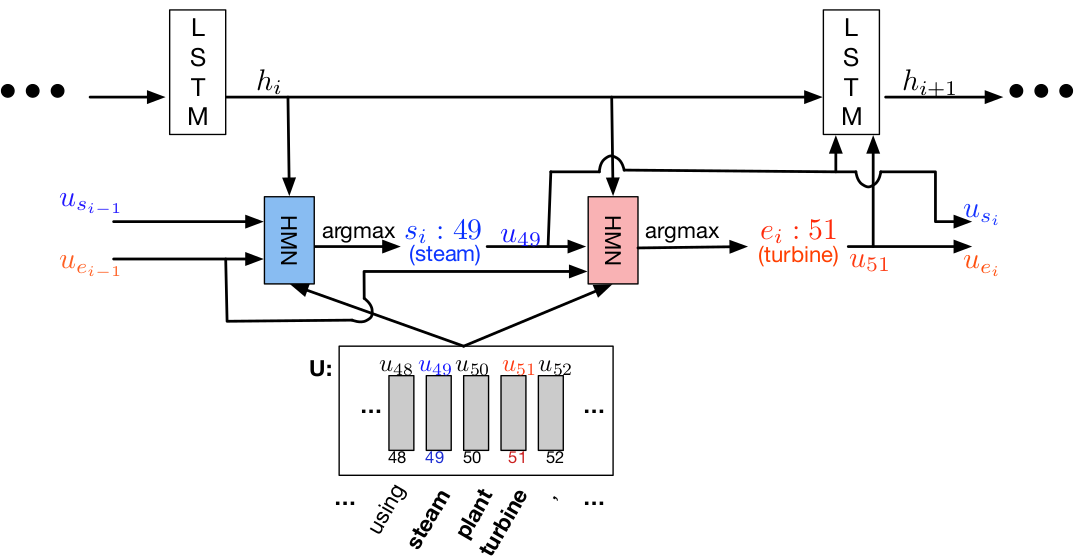
\includegraphics[width=1.0\linewidth]{dcn_dynamic_decoder.png}
    \caption{Dynamic decoder}
\end{figure}

$s_{i-1}$和$e_{i-1}$指的是第$i-1$次迭代所预测答案的起始位置和终止位置,
$u_{s_{i-1}},u_{e_{i-1}}$指的是第$i-1$次迭代所预测答案的起始位置和终止位置的那个单词在
协同注意力层输出矩阵$U$的向量表示。
\begin{gather}
s_i=\underset{t}{argmax}(\alpha_1,\cdots,\alpha_m)\notag \\
e_i=\underset{t}{argmax}(\beta_1,\cdots,\beta_m) \notag
\end{gather}
其中$\alpha_t$和$\beta_t$代表文章中第$t$个单词作为答案起始位置和终止位置的分数
$\alpha_t$和$\beta_t$的计算方式为:
\begin{gather}
    \alpha_t=\text{HMN}_{start}(u_t,h_i,u_{s_{i-1}},u_{e_{i-1}}) \notag \\
    h_i=\text{LSTM}_{dec}(h_{i-1},u_{s_{i-1}},u_{e_{i-1}}) \notag 
\end{gather}

$h_{i-1}$是第$i-1$次迭代时解码端的LSTM的隐藏状态,$u_t$是文章中第$t$个单词在$U$中的向量表示。
利用$h_{i-1},u_{s_{i-1}},u_{e_{i-1}}$计算出第$i$次迭代时LSTM的隐藏状态$h_i$,然后利用$h_i$以及
文章中每一个单词在$U$中的向量表示通过三层HMN网络计算出$\alpha$,$\alpha$的每一个值表示的就是文章中
每一个单词在第$i$次迭代作为答案起始位置的分数。

注意$\beta_t=\text{HMN}_{end}(u_t,h_i,u_{s_i},u_{e_{i-1}})$





\textbf{\kaishu \zihao{5} BiDirectional Attention Flow}
文献\upcite{Bidirectional attention flow for machine comprehension}提出一种双向注意力流模型,简称BiDAF。
首先在不同的语义粒度上表示文本,包括字符层面、单词层面、以及上下文层面。然后将问题或者段落的上下文表示送入到注意力流层。
注意力流层不同于之前流行的注意力机制
\begin{enumerate}
    \item 对于段落中每一个单词与问题计算得到的注意力结果,将它与前一层的这个单词的上下文表示连接然后流向后面的建模层
    \item 利用一种无记忆的机制,虽然类似于Bahdanau注意力\upcite{neural machine translation by jointly learning to align and translate},
对于段落的每一个时间步都会计算注意力,但是每一步计算的注意力是仅仅是关于段落和问题当前时刻的单词,与前面的时刻或后面的时刻计算的注意力都无关
    \item 不像之前的论文\upcite{Machine comprehension using match-lstm and answer pointer}仅仅
计算段落对问题的注意力,而忽视了问题对段落的注意力。
\end{enumerate}

之前的论文注意力机制大多借鉴于Bahdanau注意力\upcite{neural machine translation by jointly learning to align and translate},这种注意力运算机制的特点
就是说将段落中每一个单词的上下文表示和问题的上下文表示
做注意力的运算,计算的结果作为下一个单词做注意力计算的输入。但是这种计算方式显然前一时间步计算得到的注意力的结果会影响
下一时间步注意力的计算,也就是说这种注意力的计算方式在时间上来讲是动态的。而BiDAF在计算注意力时对于段落中
当前时间步的单词和问题计算注意力的结果不会参与下一时间步的单词计算注意力。这种机制简化了注意力的计算流程,使得注意力流层和后面的
建模层分隔开来,注意力流层会更加的专注于计算注意力,而且计算先前时间步计算的注意力出现偏差,也不会影响后面计算注意力。

具体的,输入给注意力流层的是上下文嵌入表示层的输出$C$和$Q$,其中$C\in R^{2d\times T}$是整个段落的上下文表示,
$Q\in R^{2d\times J}$是问题的上下文表示,$T$代表段落的长度,$J$代表问题的长度。
首先计算相似性矩阵$S$:
\begin{gather}
    S_{tj}=\alpha(C_{:t},Q_{:j}) \in R \notag \\ 
    \alpha(c,q)=w_{(S)}^T[c;q;c\circ q] \notag
\end{gather}

$\alpha$是编码两个向量$C$和$Q$相关性的函数,$w_{(S)}^T\in R^{6d}$是可训练的权重参数,$\circ$表示点乘。
$S\in R^{T\times J},S_{t:}\in R^{J},S_{:j}\in R_{T}$,每一行表示的段落中的一个单词对问题的相关度,每一列
表示的是问题的一个单词对整个段落的相关度。
接下来利用$S$计算两个方向的注意力,对于段落对问题的注意力C2Q,计算方式如下:
\begin{gather}
    a_t=softmax(S_{t:}) \notag\\
    \widetilde{Q}_{:t}=\sum_{j=1}^{J}a_{tj}Q_{:j}\notag
\end{gather}

$\widetilde{C}\in R^{2d\times T}$,Q2C的注意力的计算方式如下:
\begin{gather}
    b=softmax(max_{col}(S))\in R^T \notag \\
    \widetilde{q}=\sum_{t=1}^{T}b_tC_{:t} \notag 
\end{gather}
$S$的第$i$行的最大值那一列$j$表示的是段落中第$i$个单词和问题中第$j
$个单词之间的相关度最高,所以$\widetilde{q}$表示的就是段落中所有关于问题相关度最高的
单词的加权求和,这种计算方式略去了那些段落中关于问题不重要的单词。然后将$\widetilde{q}$在列的维度上
重复$T$次得到$\widetilde{Q}\in R^{2d\times T}$。

最后将计算的注意力结果$\widetilde{Q},\widetilde{C}$以及段落的上下文表示
按照$[P;\widetilde{P};p\circ\widetilde{P};P\circ\widetilde{Q}]\in R^{8d\times T}$这种方式连接,作为下一层建模层的输入。
可以看出计算出来的注意力流向了下一层,避免由于过早的把段落和文本概括为一个固定长度的向量导致信息的损失。

\textbf{\songti \zihao{5} R-Net}
文献\upcite{RNet}提出一种门控的自匹配网络。模型由四部分构成。

\begin{figure}[htbp]
    \centering
    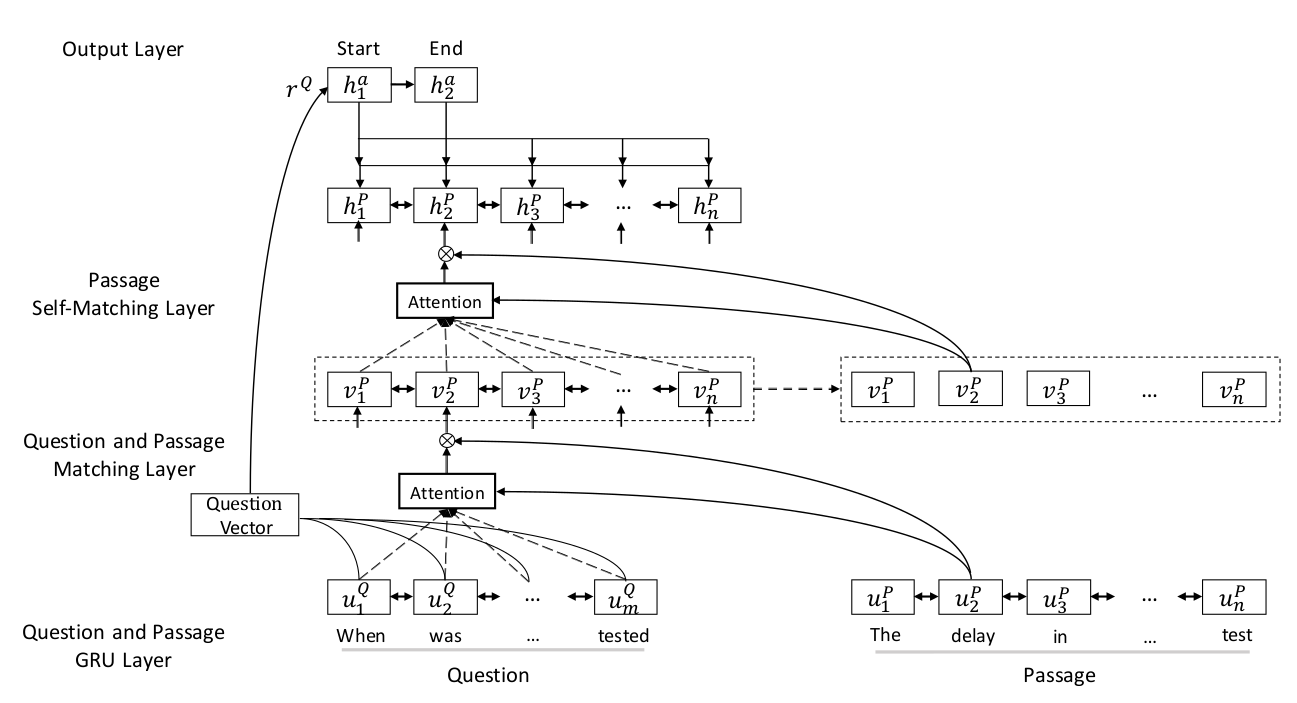
\includegraphics[width=1.0\linewidth]{rnet.png}
    \caption{Gated Self-Matching Networks structure overview.}
\end{figure}

第一部分利用双向GRU来编码文章和问题的词嵌入以及字符嵌入获得文章和问题中每一个单词的上下文表示,字符嵌入有助于解决那些未登录词典的词嵌入问题。
如图2所示,$u_1^Q,u_2^Q,\cdots,u_m^Q$表示经过BiGRU编码后的问题的上下文表示,$u_1^P,u_2^P,\cdots,u_n^P$表示文章的
上下文表示。

第二部分采用一种基于注意力的门控循环神经网络,这是基于注意力的循环神经网络的一种变体\upcite{neural machine translation by jointly learning to align and translate},
通过引入一个额外的门控单元放大那些在文章中与问题相关的部分的重要性,减小与问题无关的那部分的重要性。这种门控的思想
体现出一篇文章中只有其中一部分是与问题有关的。具体的计算方式如下:
\begin{gather}
    s_j^t=v^T\tanh(W_u^Qu_j^Q+W_u^Pu_t^P+W_v^Pv_{t-1}^P) \notag \\
    a_i^t=\exp(s_i^t)/\sum_{j=1}^{m}\exp(s_j^t)\notag \\
    c_t=\sum_{i=1}^{m}a_i^tu_i^Q \notag
\end{gather}
其中$u_j^Q$是问题的第$j$个单词的上下文表示,$u_t^P$是文章的第$t$个单词的上下文表示。$a_i^t$是
文章的第$t$个单词与问题的第$i$个单词之间的相关度。
$c_t$是将计算得到的注意力权重对整个问题加权求和得到的注意力结果。
$v_{t-1}^P$是当前层的循环神经网络上一时刻的隐藏状态。
\begin{gather}
    v_t^P=RNN(v_{t-1}^P,[u_t^P,c_t]^{*}) \notag \\
    [u_t^P,c_t]^{*}=g_t\circ [u_t^P,c_t] \notag \\
    g_t=\text{sigmoid}(W_g[u_t^P,c_t]) \notag 
\end{gather}
其中$g_t$为门控单元。

第三部分采用自匹配机制,虽然上一层的输出$v_1^P,v_2^P,\cdots,v_n^P$已经获得了关注问题的文章表示,但是一方面在SQuAD数据集中某些问题和文章
在语法和词汇上略有差异,另一方面循环神经网络实际上只能记忆有限的上下文信息,
从而导致答案中单词可能会忽视其周围单词的重要信息,
因此利用自匹配层对关注问题的文章表示做自注意力的计算。具体计算方式如下:
\begin{gather}
    s_j^t=v^T\tanh(W_v^Pv_j^P+W_v^{\widetilde{P}}v_t^P)\notag \\
    a_i^t=\exp(s_i^t)/\sum_{j=1}^{n}\exp(s_j^t)\notag \\
    c_t=\sum_{i=1}^{n}a_i^tv_i^P \notag \\    
    h_t^P=\text{BiRNN}(h_{t-1}^P,[v_t^P,c_t]^{*}) \notag \\
    [v_t^P,c_t]^{*}=g_t\circ [v_t^P,c_t] \notag \\
    g_t=\text{sigmoid}(W_g[v_t^P,c_t])\notag
\end{gather}\notag


第四部分是输出层,类似于Wang and Jiang\upcite{Machine comprehension using match-lstm and answer pointer}采用
Pointer Networks\upcite{Pointer Networks}来预测答案的起始位置和终止位置。在预测答案的起始位置时,输出层的初始状态
采用的是对问题中单词的上下文表示向量的加权求和。

\textbf{\zihao{5} QANet}
先前的模型大多使用循环神经网络来编码句子语义以及基于循环神经网络的注意力机制对文章和问题做交互。但是众所周知循环神经网络由于
序列式的特性使得训练是非常耗时的。另一方面循环神经网络由于梯度消失问题难以解决长距离依赖的情况。因此QANet\upcite{QANet}中完全
舍弃用循环神经网络作为编码器,而采用卷积神经网络与自注意力机制结合的方式再加入到transformers\upcite{Transformer}结
构中作为模型的编码器。值得一提的是虽然transformers结构已经被广泛的应用在各种NLP任务中,但是利用卷积与自注意机制的结合
是一种新的结构而且实验表明比单独的利用自注意力机制要高出2.7F1值。QANet的解码器结构与transformer的结构如图。
可以看出区别在于QANet中的编码器在输入自注意力层之前要经过几层卷积层。这里的卷积方式与传统的卷积方式不同,
采用的是深度可分离卷积\upcite{Deepwise Separable convolution}。这种卷积操作可以减少卷积层
中参数的数量。传统的卷积操作是在
每一个通道上利用卷积核同步卷积所有通道,而深度可分离卷积将传统的卷积步骤分为两个步骤。第一个步骤是
Depthwise卷积,也就是在这一步骤中每一个卷积核只负责一个通道,一个通道只由一个卷积核卷积,这样使得输入数据的特征在深度上是分离的。
第二个步骤是Pointwise卷积,将第一步输出数据在通道这一维度连接起来卷积。
完整的结构如图所示。

在输入嵌入层中一个单词的嵌入表示是词嵌入和字符嵌入的连接,其中词嵌入采用GloVe预训练的词向量\upcite{GloVe},字符嵌入采用\upcite{charCNN}
中的方式,利用卷积操作提取每一个单词的字符特征。然后将嵌入后的特征通过两层高速网络\upcite{Highway Network},输出的结果作为
嵌入编码层的输入。两个嵌入编码层的输出送入到注意力层做交互,这一层相似度矩阵的计算方式类似于BiDAF\upcite{Bidirectional attention flow for machine comprehension}
,在计算问题对文章的注意力时采用和DCN\upcite{Dynamic coattention networks for question answering}相似的计算方式,
即将文章对问题的注意力也同时考虑进去。注意力层的输出采用\upcite{Bidirectional attention flow for machine comprehension}
的思想,将文章对问题的注意力流向后面的层以减少过早加权和后的损失。然后将输出通过几层模型编码层,模型编码层后三层的输出分别作为
输入层的输入来分别的预测答案的起始位置的概率和终止位置的概率。输出层的设计是根据具体任务的,通过修改输出层,整个QANet也可以
用到其它类型的问答任务中。

数据增强



% \subsection{答案预测层的设计}
如前所述,答案预测层的设计要依据答案的形式而设计,下面介绍
各个模型在四类不同的MRC任务上的输出层设计。

1)填空型:这类任务答案的形式是预测问题中缺失的单词,而且缺失的答案来源于文章中。文献\cite{Teaching Machines to Read and Comprehend}
最早提出将问题的语义向量与关注了问题的文章的语义向量拼接成一个向量然后映射到整个词典中预测那个缺失的单词。
这种方法存在的一个问题就是不能够确保预测的单词一定是文章中的词汇,因为它是将最后的输出向量映射到整个词典中,
这就使得模型的预测准确率受到影响。指针网络(Pointer networks\upcite{Pointer Networks})模型由seq2seq模型演变而来,主要就是
为了解决输出源自于输入的问题,实现方式是利用计算的注意力的权重分布直接输出预测结果,而这种机制正适合
填空型任务以及片段选择型任务。
文献\cite{as}提出AS Reader模型正是受到指针网络的启发,对于计算得到的注意力权重分布,将其中相同单词的注意力
权值相加,最后输出具有最大权值的单词最为答案。
填空型任务模型的损失函数可以写
为$L(\theta)=-\displaystyle\frac{1}{N}\sum_{i=1}^{N}\log P_{y_i}$。
其中$\theta$为模型参数,$N$代表样本数目,$y_i$表示文章中第$i$个样本的文章中标准答案的位置。

2)多项选择型:这类任务是从多个候选答案选项中选择正确的选项。处理这种任务最简单的一种方式就是计算模型输出后的
文章的语义信息和选项之间的相似程度,相似程度最高的作为预测的选项,从而将问题变化为句子之间的语义匹配问题。
文献\cite{Co-matching}提出将问题、文章、选项一起方法模型中做交互计算输出一个向量作为输出层的输入,
输出层采用简单的输出维度是1的全连接层,输出的值代表模型对这个选型的打分值,其它的选项类似的处理,值最高的选项作为预测的答案。
最后对所有选项的打分值
做归一化作为模型的损失函数。
多项选择型任务模型的损失函数可以写为
$L(\theta)=-\displaystyle\frac{1}{N}\sum_{i=1}^{N}\sum_{j=1}^{m}\log P_{y_{j}^i}$。
其中$\theta$为模型参数,$N$代表样本数目,$m$代表选项个数,$y_{j}^i$表示第$i$个样本中第$j$个选项是正确答案。

3)片段选择型:这类任务是从文章中提取出来一段连续的单词作为答案,虽然类似于填空型任务输出来源自输入的性质,但是
不像填空型任务仅仅只是预测一个单词。因此填空型
任务答案输出层的设计不能直接用来作为片段选择型任务答案预测层。
由于提取文本的长度不固定,使得这一任务更具有挑战性。
文献\cite{MatchLSTM}受到指针网络的启发提出了两种基于指针网络的输出模型,第一种是序列式模型,利用指针网络以一种序列式的形式生成答案的每一个位置,处理过程类似于seq2seq模型的解码过程,
这种模型下答案的每一个单词可能出现在文本段落的任何一个位置,
这是因为指针网络并没有要求从输入中选择的输出具有连续性。由于答案的长度不固定,因此在段落中设置一个特殊的
位置表示答案的终止点,当预测到这个位置时终止答案的生成。
第二种是边界式模型,不同于序列式模型那样序列的生成答案的每一个位置,由于要预测的答案是一段连续的单词的组合,
因此可以利用指针网络仅仅预测答案的起始位置和终止位置。所预测答案的概率
是预测这两个位置概率的乘积,这种方式相比于
第一种更加的简单而且测试结果表明更加高效。

\noindent 边界式模型的这种设计思想也被后来很多MRC模型采纳。如RNet\upcite{RNet}采用几乎一样的边界式
模型,只不过解码端的初始状态
采用的是对问题的语义向量加权求和。尽管边界式模型简单有效,但是在文章中可能有些文本片段与标准答案相似,比如初始位置一样,
那么边界式模型有可能陷入极值的情况从而提取错误的文本片段。为了处理这个问题,DCN\upcite{Dynamic coattention networks for question answering}
模型提出一种动态迭代的指针网络作为解码端,利用上一次预测的答案的起始位置和终止位置以及解码端当前的状态来重新评估
下一次预测答案的起始位置和终止位置。多次迭代后选取所有迭代次数中概率最大的情形作为预测答案。
片段选择任务模型的损失函数可以写为
$L(\theta)=-\displaystyle\frac{1}{N}\sum_{i=1}^{N}\log P_{y_i^s}^S+\log P_{y_i^e}^E$。
其中$\theta$为模型参数,$N$代表样本数目,$y_i^s$表示第$i$个样本中标准答案的起始位置在文章中的位置,
$y_i^e$表示第$i$个样本中标准答案的终止位置在文章中的位置。
如果考虑到不可回答的问题,如数据集SQuAD 2.0\upcite{SQuAD2},还需要额外在输出层加上一个输出维度是1的全连接层。
此时的损失函数可以写为
$L(\theta)=-\displaystyle\frac{1}{N}\sum_{i=1}^{N}\log P_{y_i^s}^S+\log P_{y_i^e}^E+\log P_{y_i^u}^U$。
其中$y_i^u$表示第$i$个样本中的问题是不可回答的问题

4)自由答案型:这类任务的答案形式已经不再是原文中某段文本,而是需要根据文章和问题生成符号语法规范的答案语句。
这类任务对答案生成模块的能力要求较高。
文献\cite{CoQA}采用三种模型在在CoQA数据集上进行实验。
第一种是传统的seq2seq模型,第二种是Pointer-Generator Network\cite{PGNet},简称PGNet。
这个模型最早提出来用在文本摘要领域,模型结合了seq2seq的生成机制以及
指针网络的拷贝机制,使得模型既能生成单词又能在原文中拷贝单词,实验结果表明该模型的效果优于传统的seq2seq模型。
第三种是DrQA+PGNet模型,其中DrQA\cite{DrQA}是类似于上述
BiDAF\upcite{Bidirectional attention flow for machine comprehension},
RNet\upcite{RNet}等模型的片段抽取模块。整个模型的思想是
先利用片段提取模块从文章中提取中与问题最相关的一段文本,然后利用答案生成模块在这个被抽取出来的文本上
生成答案。这种(提取模块+生成模块)模型在其它的生成模型中如SNet\upcite{SNet}等广泛使用。
实验结果也表明这种模型的效果是最好的。







\subsection{小结}
本章是论文的核心部分,首先介绍了神经机器阅读理解模型的结构,
涉及的技术如注意力机制以及相关的模型。
然后介绍了目前流行的几种预训练模型,最后对于不同的MRC任务分别介绍了各自输出层的
设计。

在预训练模型的基础上利用具体任务的数据微调模型,
即只需要稍微添加简单的输出层即可达到很好的效果。但是预训练模型只是给了更好的初始化参数,
如果想要进一步提升模型的性能还需要在其基础上根据具体的任务设计一个更好的模型。如文献\cite{DCMN}
利用BERT作为编码器同时采用文献\cite{Co-matching}提出的co-matching方法提出了DCMN模型,在RACE\upcite{RACE}
数据集上达到了很高的准确率。文献\cite{DCMN+}在原有的DCMN模型的基础上提出了DCMN+模型,主要是增加了
句子选择模块和答案交互模块,再一次提升了模型的性能。文献\cite{Retrospective}提出一种
回顾式阅读器(Retropective Reader,Retro-Reader)模型,
以ALBERT作为编码器。Retro-Reader分为两个模块,略读模块和精读模块,主要目的就是模仿人类阅读习惯:
略读模块先阅读文章和问题然后给出初步判断问题是否可以回答,精读模块用于鉴定可回答性,
在可回答的前提下给出答案,在SQuAD 2.0\upcite{SQuAD2}数据集上显著优于其它模型。

因此可以看到如何利用预训练模型结合具体任务改进模型的结构是至关重要的。
%\end{multicols}





\section{总结与展望}
本文从机器阅读理解任务的定义出发,首先介绍了不同任务下的数据集以及相应的评估标准。
然后对神经机器阅读理解模型进行了分析与研究,主要涉及模型
的整体框架以及所用到的方法如注意力机制、推理结构等。同时也总结了
目前一些主流的预训练模型,分析了它们之间的差异,列举了一些在预训练模型的基础上改进
的模型。通过各个模型的实验对比结果可以看到基于预训练模型的模型性能要显著的优于传统的仅仅基于
注意力机制的模型。

机器阅读理解赋予了计算机阅读理解文本的能力,在搜索、对话、医疗以及教育领域都有着广阔的应用空间。
但是目前机器阅读理解仍然存在一些难题,
1)基于注意力机制的匹配模型大多是浅层的语义匹配模型,基于多跳结构的推理模式还过于单一,而
阅读理解是需要深层次的推理过程才能更好的理解文章,让模型具有较强的推理能力至关重要。

2)目前机器阅读理解领域的数据集大多是通用领域方向的,而设计专业领域数据集也尤为重要,更重要的是
这些适用于通用领域数据集的模型未必在专业领域有一样的性能。

3)生成答案的技术还需要进一步提升,回顾目前机器阅读理解领域的数据集以及相应的模型,
大多集中于片段选择式问答且模型准确度很高甚至超过人类水平。
而对于自由答案型这种需要生成答案的模型效果很差,有些模型直接将生成式问题转为抽取式问题,主要原因
在于生成答案模块对模型要求变得更高。

4)目前机器阅读理解主要集中于非结构化的文本领域,而
还有许多其它结构,不同模态的数据如表格、视频、音频、图片等,
多模态阅读理解模型也是未来的发展方向之一。






\begin{thebibliography}{99}
    \bibitem{lstm}Sepp Hochreiter and Jürgen Schmidhuber. Long short-term memory. Neural computation, 9(8):
    1735–1780, 1997.

    \bibitem{BLEU}Kishore Papineni, Salim Roukos, Todd Ward, and Wei-Jing Zhu. Bleu: a method for au-
    tomatic evaluation of machine translation. In Proceedings of the 40th Annual Meeting on
    Association for Computational Linguistics, pages 311–318. Association for Computational
    Linguistics, 2002.
    \bibitem{ROUGE}Chin-Yew Lin. Rouge: A package for automatic evaluation of summaries. Text Summariza-
    tion Branches Out, 2004.

    \bibitem{Maxout Network}Goodfellow, I.J., Warde-Farley, D., Mirza, M., Courville, A., Bengio, Y.: Maxout networks.
    arXiv preprint arXiv:1302.4389 (2013)

    \bibitem{word2vec}Mikolov T,Sutskever I,Chen K,et al.Distributed represen-
    tations of words and phrases and their compositionality[C]//
    Advances in Neural Information Processing Systems,
    2013:3111-3119.

    \bibitem{GloVe}Jeffrey Pennington, Richard Socher, and Christopher D. Manning. Glove: Global vectors for
    word//w representation. In Empirical Methods in Natural Language Processing (EMNLP), pp.
    1532–1543, 2014.

    \bibitem{neural machine translation by jointly learning to align and translate}Dzmitry Bahdanau, Kyunghyun Cho, and Yoshua Bengio. Neural machine translation by jointly
    learning to align and translate. ICLR, 2015.

    \bibitem{memory network}J. Weston, S. Chopra, and A. Bordes. Memory networks. In International Conference on
    Learning Representations (ICLR), 2015.

    \bibitem{Highway Network}Srivastava, R.K., Greff, K., Schmidhuber, J.: Highway networks.
    arXiv preprint
    arXiv:1505.00387 (2015)

    \bibitem{MemN2N}Sainbayar Sukhbaatar, Jason Weston, Rob Fergus, et al. End-to-end memory networks. In
    Advances in neural information processing systems, pages 2440–2448, 2015.

    \bibitem{Teaching Machines to Read and Comprehend}Hermann, K.M., Kocisky, T., Grefenstette, E., Espeholt, L., Kay, W., Suleyman, M., Blun-
    som, P.: Teaching machines to read and comprehend. In: Advances in Neural Information
    Processing Systems, pp. 1693–1701 (2015)

    \bibitem{AR}Danqi Chen, Jason Bolton, and Christopher D Manning. A thorough examination of the
    cnn/daily mail reading comprehension task. In Proceedings of the 54th Annual Meeting of
    the Association for Computational Linguistics (Volume 1: Long Papers), volume 1, pages
    2358–2367, 2016.

    \bibitem{ASR}Rudolf Kadlec, Martin Schmid, Ondřej Bajgar, and Jan Kleindienst. Text understanding
    with the attention sum reader network. In Proceedings of the 54th Annual Meeting of the
    Association for Computational Linguistics (Volume 1: Long Papers), volume 1, pages 908–
    918, 2016.

    \bibitem{IAReader}Alessandro Sordoni, Philip Bachman, Adam Trischler, and Yoshua Bengio. Iterative alternat-
    ing neural attention for machine reading. arXiv preprint arXiv:1606.02245, 2016.

    \bibitem{SQuAD1}Pranav Rajpurkar, Jian Zhang, Konstantin Lopyrev, and Percy Liang. SQuAD: 100,000+ questions
    for machine comprehension of text. In Proceedings of the Conference on Empirical Methods in
    Natural Language Processing, 2016.

    \bibitem{sentinel vector}Merity, S., Xiong, C., Bradbury, J., Socher, R.: Pointer sentinel mixture models. arXiv
    preprint arXiv:1609.07843 (2016)

    \bibitem{Machine comprehension using match-lstm and answer pointer}Wang, S., Jiang, J.: Machine comprehension using match-lstm and answer pointer. arXiv
    preprint arXiv:1608.07905 (2016)

    \bibitem{Dynamic coattention networks for question answering}Xiong, C., Zhong, V., Socher, R.: Dynamic coattention networks for question answering.
    arXiv preprint arXiv:1611.01604 (2016)

    \bibitem{Bidirectional attention flow for machine comprehension}Seo, M., Kembhavi, A., Farhadi, A., Hajishirzi, H.: Bidirectional attention flow for machine
    comprehension. arXiv preprint arXiv:1611.01603 (2016)
    
    \bibitem{RNet}Wang, W., Yang, N., Wei, F., Chang, B., Zhou, M.: Gated self-matching networks for
    reading comprehension and question answering. In: Proceedings of the 55th Annual Meet-
    ing of the Association for Computational Linguistics (Volume 1: Long Papers), vol. 1, pp.
    189–198 (2017)

    \bibitem{Reasonet}Shen, Y., Huang, P.S., Gao, J., Chen, W.: Reasonet: Learning to stop reading in machine
    comprehension. In: Proceedings of the 23rd ACM SIGKDD International Conference on
    Knowledge Discovery and Data Mining, pp. 1047–1055. ACM (2017)

    \bibitem{GAReader}Bhuwan Dhingra, Hanxiao Liu, Zhilin Yang, William Cohen, and Ruslan Salakhutdinov.
    Gated-attention readers for text comprehension. In Proceedings of the 55th Annual Meeting
    of the Association for Computational Linguistics (Volume 1: Long Papers), pages 1832–1846,
    2017.

    \bibitem{DrQA}Danqi Chen, Adam Fisch, Jason Weston, and
    Antoine Bordes. 2017. Reading Wikipedia
    to answer open-domain questions. In Asso-
    ciation for Computational Linguistics (ACL),
    pages 1870–1879. Vancouver, Canada.

    \bibitem{FusionNet}Hsin-Yuan Huang, Chenguang Zhu, Yelong Shen, Weizhu Chen.
    FusionNet: Fusing via Fully-Aware Attention with Application to Machine Comprehension. In Proceedings of the 
    Sixth International Conference on Learning Representations (ICLR), 2018.

    \bibitem{MatchLSTM}Shuohang Wang and Jing Jiang. Learning natural language inference with LSTM. In Proceedings of
    the Conference on the North American Chapter of the Association for Computational Linguistics,
    2016.
    \bibitem{Pointer Networks}Oriol Vinyals, Meire Fortunato, and Navdeep Jaitly. Pointer networks. In Proceedings of the Con-
    ference on Advances in Neural Information Processing Systems, 2015.
    \bibitem{RACE}Guokun Lai, Qizhe Xie, Hanxiao Liu, Yiming Yang, and Eduard Hovy. Race: Large-scale
    reading comprehension dataset from examinations. In Proceedings of the 2017 Conference
    on Empirical Methods in Natural Language Processing, pages 785–794, 2017.
    \bibitem{SQuAD2}Rajpurkar, P., Jia, R., Liang, P.: Know what you don’t know: Unanswerable questions for
    squad. arXiv preprint arXiv:1806.03822 (2018)
    \bibitem{CBT}Hill, F., Bordes, A., Chopra, S., Weston, J.: The goldilocks principle: Reading children’s
    books with explicit memory representations. arXiv preprint arXiv:1511.02301 (2015)
    \bibitem{QANet}Yu, A.W., Dohan, D., Luong, M.T., Zhao, R., Chen, K., Norouzi, M., Le, Q.V.: Qanet:
    Combining local convolution with global self-attention for reading comprehension. arXiv
    preprint arXiv:1804.09541 (2018)
    \bibitem{CoQA}Siva Reddy, Danqi Chen, and Christopher D Manning. Coqa: A conversational question answering
    challenge. arXiv preprint arXiv:1808.07042, 2018.
    \bibitem{MS marco}Nguyen, T., Rosenberg, M., Song, X., Gao, J., Tiwary, S., Majumder, R., Deng, L.:
    Ms marco: A human generated machine reading comprehension dataset. arXiv preprint
    arXiv:1611.09268 (2016)
    \bibitem{NarrativeQA}Kočiskỳ, T., Schwarz, J., Blunsom, P., Dyer, C., Hermann, K.M., Melis, G., Grefenstette,
    E.: The narrativeqa reading comprehension challenge. Transactions of the Association of
    Computational Linguistics 6, 317–328 (2018)
    \bibitem{Transformer}Ashish Vaswani, Noam Shazeer, Niki Parmar, Jakob Uszkoreit, Llion Jones, Aidan N Gomez,
    Lukasz Kaiser, and Illia Polosukhin. Attention is all you need. In Neural Information Processing
    Systems, 2017b.

    \bibitem{Deepwise Separable convolution}François Chollet. Xception: Deep learning with depthwise separable convolutions.
    abs/1610.02357, 2016.
    \bibitem{ELMo}Peters, M.E., Neumann, M., Iyyer, M., Gardner, M., Clark, C., Lee, K., Zettlemoyer, L.:
    Deep contextualized word representations. arXiv preprint arXiv:1802.05365 (2018)
    \bibitem{GPT}Radford, A., Narasimhan, K., Salimans, T., Sutskever, I.: Improving language understand-
    ing with unsupervised learning. Tech. rep., Technical report, OpenAI (2018)
    \bibitem{BERT}Devlin, J., Chang, M.W., Lee, K., Toutanova, K.: Bert: Pre-training of deep bidirectional
    transformers for language understanding. arXiv preprint arXiv:1810.04805 (2018)

    \bibitem{XLNet}Zhilin Yang, Zihang Dai, Yiming Yang, Jaime Carbonell, Ruslan Salakhutdinov, and Quoc V
    Le. XLNet: Generalized autoregressive pretraining for language understanding. arXiv preprint
    arXiv:1906.08237, 2019.

    \bibitem{RoBERTa}Yinhan Liu, Myle Ott, Naman Goyal, Jingfei Du, Mandar Joshi, Danqi Chen, Omer Levy, Mike
    Lewis, Luke Zettlemoyer, and Veselin Stoyanov. RoBERTa: A robustly optimized BERT pre-
    training approach. arXiv preprint arXiv:1907.11692, 2019.

    \bibitem{ALBERT}Zhenzhong Lan, Mingda Chen, Sebastian Goodman,
    Kevin Gimpel, Piyush Sharma, and Radu Soricut.
    2020. ALBERT: A lite BERT for self-supervised
    learning of language representations. In ICLR.
    \bibitem{VQACo}Jiasen Lu, Jianwei Yang, Dhruv Batra, and Devi Parikh. Hierarchical question-image co-attention
    for visual question answering. arXiv preprint arXiv:1606.00061, 2016.
    \bibitem{UNILM}Li Dong, Nan Yang, Wenhui Wang, Furu Wei, Xiaodong Liu,
    Yu Wang, Jianfeng Gao, Ming Zhou, and Hsiao-Wuen Hon.
    Unified language model pre-training for natural language un-
    derstanding and generation. In NeurIPS, pages 13042–13054,
    2019.
    \bibitem{Co-matching}Shuohang Wang, Mo Yu, Jing Jiang, and Shiyu Chang.
    2018. A Co-Matching Model for Multi-choice
    Reading Comprehension. In Proceedings of the 56th
    Annual Meeting of the Association for Computa-
    tional Linguistics (Volume 2: Short Papers), pages
    746–751. Association for Computational Linguis-
    tics.
    \bibitem{PGNet}Abigail See, Peter J. Liu, and Christopher D.
    Manning. 2017. Get to the point: Summa-
    rization with pointer-generator networks. In
    Annual Meeting of the Association for Compu-
    tational Linguistics (ACL), pages 1073–1083.
    Vancouver, Canada.
    \bibitem{SNet}Chuanqi Tan, Furu Wei, Nan Yang, Bowen Du, Weifeng Lv, and Ming Zhou. S-net: From
    answer extraction to answer synthesis for machine reading comprehension. In Thirty-Second
    AAAI Conference on Artificial Intelligence, 2018.






\end{thebibliography}
\end{multicols}








\end{document}